% Options for packages loaded elsewhere
\PassOptionsToPackage{unicode}{hyperref}
\PassOptionsToPackage{hyphens}{url}
%
\documentclass[
  man]{apa6}
\usepackage{amsmath,amssymb}
\usepackage{lmodern}
\usepackage{iftex}
\ifPDFTeX
  \usepackage[T1]{fontenc}
  \usepackage[utf8]{inputenc}
  \usepackage{textcomp} % provide euro and other symbols
\else % if luatex or xetex
  \usepackage{unicode-math}
  \defaultfontfeatures{Scale=MatchLowercase}
  \defaultfontfeatures[\rmfamily]{Ligatures=TeX,Scale=1}
\fi
% Use upquote if available, for straight quotes in verbatim environments
\IfFileExists{upquote.sty}{\usepackage{upquote}}{}
\IfFileExists{microtype.sty}{% use microtype if available
  \usepackage[]{microtype}
  \UseMicrotypeSet[protrusion]{basicmath} % disable protrusion for tt fonts
}{}
\makeatletter
\@ifundefined{KOMAClassName}{% if non-KOMA class
  \IfFileExists{parskip.sty}{%
    \usepackage{parskip}
  }{% else
    \setlength{\parindent}{0pt}
    \setlength{\parskip}{6pt plus 2pt minus 1pt}}
}{% if KOMA class
  \KOMAoptions{parskip=half}}
\makeatother
\usepackage{xcolor}
\usepackage{graphicx}
\makeatletter
\def\maxwidth{\ifdim\Gin@nat@width>\linewidth\linewidth\else\Gin@nat@width\fi}
\def\maxheight{\ifdim\Gin@nat@height>\textheight\textheight\else\Gin@nat@height\fi}
\makeatother
% Scale images if necessary, so that they will not overflow the page
% margins by default, and it is still possible to overwrite the defaults
% using explicit options in \includegraphics[width, height, ...]{}
\setkeys{Gin}{width=\maxwidth,height=\maxheight,keepaspectratio}
% Set default figure placement to htbp
\makeatletter
\def\fps@figure{htbp}
\makeatother
\setlength{\emergencystretch}{3em} % prevent overfull lines
\providecommand{\tightlist}{%
  \setlength{\itemsep}{0pt}\setlength{\parskip}{0pt}}
\setcounter{secnumdepth}{-\maxdimen} % remove section numbering
% Make \paragraph and \subparagraph free-standing
\ifx\paragraph\undefined\else
  \let\oldparagraph\paragraph
  \renewcommand{\paragraph}[1]{\oldparagraph{#1}\mbox{}}
\fi
\ifx\subparagraph\undefined\else
  \let\oldsubparagraph\subparagraph
  \renewcommand{\subparagraph}[1]{\oldsubparagraph{#1}\mbox{}}
\fi
\newlength{\cslhangindent}
\setlength{\cslhangindent}{1.5em}
\newlength{\csllabelwidth}
\setlength{\csllabelwidth}{3em}
\newlength{\cslentryspacingunit} % times entry-spacing
\setlength{\cslentryspacingunit}{\parskip}
\newenvironment{CSLReferences}[2] % #1 hanging-ident, #2 entry spacing
 {% don't indent paragraphs
  \setlength{\parindent}{0pt}
  % turn on hanging indent if param 1 is 1
  \ifodd #1
  \let\oldpar\par
  \def\par{\hangindent=\cslhangindent\oldpar}
  \fi
  % set entry spacing
  \setlength{\parskip}{#2\cslentryspacingunit}
 }%
 {}
\usepackage{calc}
\newcommand{\CSLBlock}[1]{#1\hfill\break}
\newcommand{\CSLLeftMargin}[1]{\parbox[t]{\csllabelwidth}{#1}}
\newcommand{\CSLRightInline}[1]{\parbox[t]{\linewidth - \csllabelwidth}{#1}\break}
\newcommand{\CSLIndent}[1]{\hspace{\cslhangindent}#1}
\ifLuaTeX
\usepackage[bidi=basic]{babel}
\else
\usepackage[bidi=default]{babel}
\fi
\babelprovide[main,import]{english}
% get rid of language-specific shorthands (see #6817):
\let\LanguageShortHands\languageshorthands
\def\languageshorthands#1{}
% Manuscript styling
\usepackage{upgreek}
\captionsetup{font=singlespacing,justification=justified}

% Table formatting
\usepackage{longtable}
\usepackage{lscape}
% \usepackage[counterclockwise]{rotating}   % Landscape page setup for large tables
\usepackage{multirow}		% Table styling
\usepackage{tabularx}		% Control Column width
\usepackage[flushleft]{threeparttable}	% Allows for three part tables with a specified notes section
\usepackage{threeparttablex}            % Lets threeparttable work with longtable

% Create new environments so endfloat can handle them
% \newenvironment{ltable}
%   {\begin{landscape}\centering\begin{threeparttable}}
%   {\end{threeparttable}\end{landscape}}
\newenvironment{lltable}{\begin{landscape}\centering\begin{ThreePartTable}}{\end{ThreePartTable}\end{landscape}}

% Enables adjusting longtable caption width to table width
% Solution found at http://golatex.de/longtable-mit-caption-so-breit-wie-die-tabelle-t15767.html
\makeatletter
\newcommand\LastLTentrywidth{1em}
\newlength\longtablewidth
\setlength{\longtablewidth}{1in}
\newcommand{\getlongtablewidth}{\begingroup \ifcsname LT@\roman{LT@tables}\endcsname \global\longtablewidth=0pt \renewcommand{\LT@entry}[2]{\global\advance\longtablewidth by ##2\relax\gdef\LastLTentrywidth{##2}}\@nameuse{LT@\roman{LT@tables}} \fi \endgroup}

% \setlength{\parindent}{0.5in}
% \setlength{\parskip}{0pt plus 0pt minus 0pt}

% Overwrite redefinition of paragraph and subparagraph by the default LaTeX template
% See https://github.com/crsh/papaja/issues/292
\makeatletter
\renewcommand{\paragraph}{\@startsection{paragraph}{4}{\parindent}%
  {0\baselineskip \@plus 0.2ex \@minus 0.2ex}%
  {-1em}%
  {\normalfont\normalsize\bfseries\itshape\typesectitle}}

\renewcommand{\subparagraph}[1]{\@startsection{subparagraph}{5}{1em}%
  {0\baselineskip \@plus 0.2ex \@minus 0.2ex}%
  {-\z@\relax}%
  {\normalfont\normalsize\itshape\hspace{\parindent}{#1}\textit{\addperi}}{\relax}}
\makeatother

\makeatletter
\usepackage{etoolbox}
\patchcmd{\maketitle}
  {\section{\normalfont\normalsize\abstractname}}
  {\section*{\normalfont\normalsize\abstractname}}
  {}{\typeout{Failed to patch abstract.}}
\patchcmd{\maketitle}
  {\section{\protect\normalfont{\@title}}}
  {\section*{\protect\normalfont{\@title}}}
  {}{\typeout{Failed to patch title.}}
\makeatother

\usepackage{xpatch}
\makeatletter
\xapptocmd\appendix
  {\xapptocmd\section
    {\addcontentsline{toc}{section}{\appendixname\ifoneappendix\else~\theappendix\fi\\: #1}}
    {}{\InnerPatchFailed}%
  }
{}{\PatchFailed}
\keywords{language input; blind children; LENA}
\DeclareDelayedFloatFlavor{ThreePartTable}{table}
\DeclareDelayedFloatFlavor{lltable}{table}
\DeclareDelayedFloatFlavor*{longtable}{table}
\makeatletter
\renewcommand{\efloat@iwrite}[1]{\immediate\expandafter\protected@write\csname efloat@post#1\endcsname{}}
\makeatother
\usepackage{csquotes}
\usepackage{float}
\floatplacement{figure}{H}
\ifLuaTeX
  \usepackage{selnolig}  % disable illegal ligatures
\fi
\IfFileExists{bookmark.sty}{\usepackage{bookmark}}{\usepackage{hyperref}}
\IfFileExists{xurl.sty}{\usepackage{xurl}}{} % add URL line breaks if available
\urlstyle{same} % disable monospaced font for URLs
\hypersetup{
  pdftitle={Comparing Language Input in Homes of Young Blind and Sighted Children: Insights from Daylong Recordings},
  pdfauthor={Erin Campbell1,2, Lillianna Righter1,3, Eugenia Lukin1,3, \& Elika Bergelson1,3},
  pdflang={en-EN},
  pdfkeywords={language input; blind children; LENA},
  hidelinks,
  pdfcreator={LaTeX via pandoc}}

\title{Comparing Language Input in Homes of Young Blind and Sighted Children: Insights from Daylong Recordings}
\author{Erin Campbell\textsuperscript{1,2}, Lillianna Righter\textsuperscript{1,3}, Eugenia Lukin\textsuperscript{1,3}, \& Elika Bergelson\textsuperscript{1,3}}
\date{}


\shorttitle{Language Input to Blind and Sighted Children}

\authornote{

Correspondence concerning this article should be addressed to Erin Campbell, 2 Silber Way, Room 513, Boston, MA 02215. E-mail: \href{mailto:eecamp@bu.edu}{\nolinkurl{eecamp@bu.edu}}

}

\affiliation{\vspace{0.5cm}\textsuperscript{1} Department of Psychology \& Neuroscience, Duke University, Durham, NC\\\textsuperscript{2} Wheelock College of Education \& Human Development, Boston University, Boston, MA\\\textsuperscript{3} Department of Psychology, Harvard University, Cambridge, MA}

\note{

\textbf{Conflicts of Interest}: The authors have no conflicts of interest to report.
\textbf{Funding}: This work was supported by the National Science Foundation CAREER grant (BCS-1844710) to EB and Graduate Research Fellowship (2019274952) to EC.

}

\begin{document}
\maketitle

\hypertarget{abstract}{%
\section{Abstract}\label{abstract}}

We compared everyday language input to young congenitally-blind children with no additional disabilities (N=15, 6--30mo., M:16mo.) and demographically-matched sighted peers (N=15, 6--31mo., M:16mo.). By studying whether the language input of blind children differs from their sighted peers, we aimed to determine whether, in principle, the language acquisition patterns observed in blind and sighted children could be explained by aspects of the speech they hear. Children wore LENA recorders to capture the auditory language environment in their homes. Speech in these recordings was then analyzed with a mix of automated and manually-transcribed measures across various subsets and dimensions of language input. These included measures of quantity (adult words), interaction (conversational turns and child-directed speech), linguistic properties (lexical diversity and mean length of utterance), and conceptual features (talk centered around the here-and-now; talk focused on visual referents that would be inaccessible to the blind but not sighted children). Overall, we found broad similarity across groups in speech quantity, interaction, and linguistic properties. The only exception was that blind children's language environments contained slightly but significantly more talk about past/future/hypothetical events than sighted children's input; both groups received equivalent quantities of ``visual'' speech input. The findings challenge the notion that blind children's language input diverges substantially from sighted children's; while the input is highly variable across children, it is not systematically so across groups, across nearly all measures. The findings suggest instead that blind children and sighted children alike receive input that readily supports their language development, with open questions remaining regarding how this input may be differentially leveraged by language learners in early childhood.

\hypertarget{introduction}{%
\section{Introduction}\label{introduction}}

The early language skills of blind children are highly variable. Some children demonstrate age-appropriate vocabulary and grammar from the earliest stages of language learning, while others experience substantial language delays (Bigelow, 1987; E. E. Campbell, Casillas, \& Bergelson, 2024; Landau \& Gleitman, 1985). By adulthood, however, blind individuals are fluent language-users, even demonstrating faster lexical processing skills than sighted adults (Loiotile, Lane, Omaki, \& Bedny, 2020; Röder, Demuth, Streb, \& Rösler, 2003; Röder, Rösler, \& Neville, 2000; though c.f., Sak-Wernicka, 2017 for discussion of possible pragmatic differences). The causes of early variability and the potential ability (or need) to ``catch up'' remain poorly understood: what could make the language learning problem different or initially more difficult for the blind child? Here, we compare the language environments of blind children to that of their sighted peers. In doing so, we begin to untangle the role that perceptual input plays in shaping children's language environment, and better understand the interlocking factors that may contribute to variability in blind children's early language abilities.

\hypertarget{why-would-input-matter}{%
\subsection{Why would input matter?}\label{why-would-input-matter}}

Among both typically-developing children and children with developmental differences, language input has been found to predict variability in language outcomes (Anderson, Graham, Prime, Jenkins, \& Madigan, 2021, 2021; Gilkerson et al., 2018; Huttenlocher, Haight, Bryk, Seltzer, \& Lyons, 1991; Huttenlocher, Waterfall, Vasilyeva, Vevea, \& Hedges, 2010; Rowe, 2008, 2012). The many ways to operationalize language input tend to be grouped into \textbf{quantity} measures and \textbf{input characteristics} (often referred to as ``quality'' measures)\footnote{We avoid the term ``quality'' here as it carries potential biases regarding linguistic norms (MacLeod \& Demers, 2023).}. Quantity can be broadly construed as the number of words or utterances a child is exposed to. At a coarse level, children who are exposed to more speech (or sign, Watkins, Pittman, \& Walden, 1998) tend to have stronger language outcomes and produce more speech themselves (Anderson et al., 2021; Bergelson et al., 2023; Gilkerson et al., 2018; Huttenlocher et al., 1991; Rowe, 2008).

Previous research suggests that the specific characteristics of language input are perhaps even more influential than quantity measures alone (Hirsh-Pasek et al., 2015; Rowe, 2012), although they are somewhat trickier to delineate and assess. Rowe and Snow (2020) categorized this space into three dimensions: interactive features (e.g., parent responsiveness, speech directed \emph{to} child vs.~overheard, conversational turn-taking), linguistic features (e.g., lexical diversity, grammatical complexity), and conceptual features (i.e., the extent to which input focuses on the \emph{here-and-now}), which we adopt here.

In terms of interactive features, previous studies have indicated that back-and-forth communicative exchanges (also known as conversational turns) between caregivers and children are predictive of better language outcomes across infancy (Donnellan, Bannard, McGillion, Slocombe, \& Matthews, 2020; Goldstein \& Schwade, 2008) and toddlerhood (Hirsh-Pasek et al., 2015; Romeo et al., 2018). Another way to quantify the extent to which caregivers and infants interact is by looking at how much speech is directed \emph{to} the child (as opposed to, for example, an overheard conversation between adults). The amount of child-directed speech in children's input (at least in Western contexts, Casillas, Brown, \& Levinson, 2020) has been linked to children's vocabulary size and lexical processing (Rowe, 2008; Shneidman, Arroyo, Levine, \& Goldin-Meadow, 2013; Weisleder \& Fernald, 2013).

Under the linguistic umbrella, we can measure the \emph{kinds} of words used (often measured as lexical diversity, type-token ratio), and the ways they are \emph{combined} (syntactic complexity, often measured by mean length of utterance). Both parameters have been found to correlate with children's language growth: sighted toddlers who are exposed to a greater diversity of words in their language input are reported to have larger vocabulary scores (Anderson et al., 2021; Hsu, Hadley, \& Rispoli, 2017; Huttenlocher et al., 2010; Rowe, 2012; Weizman \& Snow, 2001). Likewise, the diversity and complexity of syntactic constructions in parental language input has been associated with both children's vocabulary growth and structural diversity in their own productions (De Villiers, 1985; Hadley et al., 2017; Hoff, 2003; Huttenlocher, Vasilyeva, Cymerman, \& Levine, 2002; Huttenlocher et al., 2010; Naigles \& Hoff-Ginsberg, 1998).

Finally, the conceptual dimension of language input aims to capture the extent to which the language signal maps onto present objects and ongoing events in children's environments (Rowe \& Snow, 2020). As children develop, their ability to represent abstract referents improves (Bergelson \& Swingley, 2013; Kramer, Hill, \& Cohen, 1975; Luchkina, Xu, Sobel, \& Morgan, 2020). Decontextualized language input-- that is, talking about past, future, or hypothetical events, or people and items that are not currently present in the environment-- may be one contributing factor (Rowe, 2013). Greater prevalence of decontextualized language in input to toddlers has been found to predict aspects of children's own language in kindergarten and beyond (Demir, Rowe, Heller, Goldin-Meadow, \& Levine, 2015; Rowe, 2012; Uccelli, Demir-Lira, Rowe, Levine, \& Goldin-Meadow, 2019).

From this (necessarily abridged) review, it appears that many factors in the language input alone link to how sighted children learn about the world and language, but that children also learn from sensory, conceptual, and social knowledge. Many cues for word learning are visual: for example, empirical work finds that sighted children can leverage visual information like parental gaze, shared visual attention (Tomasello \& Farrar, 1986), pointing (Lucca \& Wilbourn, 2018), and the presence of salient objects in the visual field (Yu \& Smith, 2012). Because these visual cues are inaccessible to blind children, language input may take on a larger role in the discovery of word meaning (E. E. Campbell \& Bergelson, 2022). Syntactic structure in particular provides critical cues to word meaning, such as the relationship between two entities that aren't within reach, or are intrinsically unobservable or ambiguous (Gleitman, 1990). But in order to evaluate whether language input plays a larger role for blind versus sighted children's learning, it is worth first establishing whether blind and sighted children's language input differs. That is, children with different sensory access could differentially make use of the same kind of language input, or they could apply the same learning mechanisms to input with different properties--a debate carried over from work with typically-sighted children (Newport, Gleitman, \& Gleitman, 1977). Either way, characterizing the input across potentially relevant dimensions is a helpful first step.

\hypertarget{why-would-the-input-differ-between-blind-and-sighted-children}{%
\subsection{Why would the input differ between blind and sighted children?}\label{why-would-the-input-differ-between-blind-and-sighted-children}}

Speakers regularly tailor their speech to communicate efficiently with the listener (Grice, 1975). Across many contexts, research finds that parents are sensitive to their child's developmental level and tune language input accordingly (Newport et al., 1977; Snow, 1972; Vygotsky \& Cole, 1978). One example is child-directed speech, wherein parents speak to young children with exaggerated prosody and slower speech (Bernstein Ratner, 1984; Fernald, 1989; Moser et al., 2022; Newport et al., 1977), which are in some cases helpful to the young language learner (Thiessen, Hill, \& Saffran, 2005). For instance, parents tend to repeat words more often when interacting with infants than with older children or adults (Fernald \& Morikawa, 1993; Snow, 1972). Communicative tailoring is also common in language input to children with disabilities, who have been found to receive simplified, more directive language input, and less interactive input compared to typically-developing children (Dirks, Stevens, Kok, Frijns, \& Rieffe, 2020; Yoshinaga-Itano, Sedey, Mason, Wiggin, \& Chung, 2020). In other contexts, language input to children with disabilities has been shown to be more multimodal, such that parents more frequently combine communicative cues (e.g., speech and touch, Abu-Zhaya, Kondaurova, Houston, \& Seidl, 2019) when interacting with deaf children, compared to their typically-hearing peers.

In addition to tailoring communication to children's developmental level, speakers also adjust their conversation in accordance to their conversational partner's sensory access (Gergle, Kraut, \& Fussell, 2004; Grigoroglou, Edu, \& Papafragou, 2016). In a noisy environment, speakers often adapt the acoustic-phonetic features of their speech to make it easier for their interlocutor to understand them (Hazan \& Baker, 2011), demonstrating sensitivity to even temporary sensory conditions. When describing scenes, speakers tend to provide the information their listeners lack but avoid redundant visual description (Grice, 1975; Ostarek, Paridon, \& Montero-Melis, 2019). During in-lab tasks with sighted participants, participants in several studies verbally provide visually-absent cues when an object is occluded to their partner (Hawkins, Gweon, \& Goodman, 2021; Jara-Ettinger \& Rubio-Fernandez, 2021; Rubio-Fernandez, 2019). These results suggest that adults and even infants (Chiesa, Galati, \& Schmidt, 2015; Ganea et al., 2018; Senju et al., 2013) can flexibly adapt communication to the visual and auditory abilities of their partner.

Taking these results into consideration, we might expect parents of blind children to verbally compensate for missing visual input, perhaps providing more description of the child's environment. But prior research doesn't yield a clear answer. Several studies suggest differences in the conceptual features: caregivers of blind children restrict conversation to things that the blind child is currently engaged with, rather than attempt to redirect their attention to other stimuli (Andersen, Dunlea, \& Kekelis, 1993; J. Campbell, 2003; Kekelis \& Andersen, 1984; though c.f., Moore \& McConachie, 1994). Studies of naturalistic input to blind children report that parents use \emph{fewer} declaratives and \emph{more} imperatives than parents of sighted children, suggesting that blind children might be receiving less description than sighted children (Kekelis \& Andersen, 1984; Landau \& Gleitman, 1985; though c.f., Lukin, Campbell, Righter, \& Bergelson, 2023; Pérez-Pereira \& Conti-Ramsden, 2001). Other studies report that parents adapt their interactions to their children's visual abilities, albeit in specific contexts. Tadić, Pring, and Dale (2013) find that in a structured book-reading task, parents of blind children provide more descriptive utterances than parents of sighted children. Further, parents of blind children have been found to provide more tactile cues to initiate interactions or establish joint attention (Preisler, 1991; Urwin, 1983, 1984), which may serve the same social role as shared gaze in sighted children. These mixed results suggest that parents of blind children might alter language input in some domains but not others. The apparent conflict in results may be exacerbated by the difficulty of recruiting specialized populations to participate in research: the small (in most cases, single-digit) sample sizes of prior work limits our ability to generalize about any differences in the input to blind vs.~sighted infants.

\hypertarget{the-present-study}{%
\subsection{The Present Study}\label{the-present-study}}

Children can and do learn language in a variety of input scenarios (Gleitman \& Newport, 1995), but if language input differs systematically between blind infants and toddlers, capturing this variation may reveal a more nuanced picture of how infants use the input to learn language. In the present study, we examine daylong recordings of the naturalistic language environments of blind and sighted children in order to characterize the input to each group. Using both automated measures and manual transcription of these recordings, we measure input quantity (adult word count) and analyze several characteristics that have been previously suggested to be information-rich learning cues, including interaction (conversational turn count, proportion of child-directed speech), conceptual features (temporal displacement, sensory modality), and linguistic complexity (type-token ratio and mean length of utterance). Though the present study is largely exploratory, based on prior research (i.e., Andersen et al., 1993; J. Campbell, 2003; Dirks et al., 2020; Grumi et al., 2021; Kekelis \& Andersen, 1984, 1984; Lorang, Venker, \& Sterling, 2020; Moore \& McConachie, 1994; Pérez-Pereira \& Conti-Ramsden, 2001; Preisler, 1991; Charity Rowland, 1984), we predict that blind vs.~sighted children would have input featuring less interactivity (fewer conversational turns and less child-directed speech), less linguistic complexity (lower type-token ratio and shorter utterances), and conceptual content focused more on the child's locus of attention (more here-and-now speech and fewer visual words); we have no \emph{a priori} hypotheses regarding language input quantity.

\hypertarget{methods}{%
\section{Methods}\label{methods}}

\begin{table}

\caption{\label{tab:participant-characteristics}Demographic characteristics of the blind and sighted samples. For continuous variables, range and mean are provided. For categorical variables, percentages by level are provided.}
\centering
\fontsize{8}{10}\selectfont
\begin{tabular}[t]{l|l|l}
\hline
Variable & Blind (N=15) & Sighted (N=15)\\
\hline
Age (months) & 6--30,
15.8 (8.2) & 6--32,
16.1 (8.1)\\
\hline
Sex & Female: 44\% & Female: 44\%\\
\hline
 & Male: 56\% & Male: 56\%\\
\hline
Number of Older Siblings & 0--2,
0.5 (0.8) & 0--3,
1.1 (1)\\
\hline
Race & American Indian or Alaska Native: 6\% & American Indian or Alaska Native: 0\%\\
\hline
 & Black or African American: 6\% & Black or African American: 6\%\\
\hline
 & Mixed: 19\% & Mixed: 6\%\\
\hline
 & White: 69\% & White: 44\%\\
\hline
 & unknown: 0\% & unknown: 44\%\\
\hline
Maternal Education & Some college: 19\% & Some college: 6\%\\
\hline
 & Associate's degree: 6\% & Associate's degree: 12\%\\
\hline
 & Bachelor's degree: 31\% & Bachelor's degree: 56\%\\
\hline
 & Graduate degree: 44\% & Graduate degree: 6\%\\
\hline
Ethnicity & Hispanic or Latino: 19\% & Hispanic or Latino: 0\%\\
\hline
 & Not Hispanic or Latino: 81\% & Not Hispanic or Latino: 50\%\\
\hline
 & unknown: 0\% & unknown: 50\%\\
\hline
\end{tabular}
\end{table}

\hypertarget{participants}{%
\subsection{Participants}\label{participants}}

This study included 15 congenitally-blind infants and their families\footnote{One family contributed two recordings for the same blind child. In the present study, we used only the first recording from that participant.}. To be eligible, participants had to be 6--30 months old, have severe to profound visual impairment (i.e.~at most light perception), no additional disabilities (developmental delays, intellectual disabilities, or hearing loss), and be exposed to \(\geq\) 75\% English at home. Blind participants were recruited through ophthalmologist referral, preschools, early intervention programs, social media, and word of mouth. Blindness in our sample was caused by a range of conditions, including cataracts (n=3), Leber's Congenital Amaurosis (n=1), Microphthalmia (n=2), Ocular albinism (n=2), Optic Nerve Hypoplasia (n=2), Retinal Detachments (n=1), and Retinopathy of Prematurity (n=1). Etiology was unknown in 2 participants, and 2 participants had multiple contributing conditions. Caregivers were also asked to complete a demographics survey and the MacArthur-Bates Communicative Development Inventory (CDI, Fenson et al., 1994) within one week of the home language recording.

To control for the wide age range of the study, each blind participant was matched to a sighted participant, based on age (\(\pm\) 6 weeks), sex, maternal education (\(\pm\) one education level), and number of siblings (\(\pm\) 1 sibling). Sighted matches were drawn from the multiple existing corpora (Bergelson, 2015; Bergelson, Amatuni, Dailey, Koorathota, \& Tor, 2019; Ramírez-Esparza, García-Sierra, \& Kuhl, 2014; Caroline Rowland et al., 2018; VanDam et al., 2015; VanDam et al., 2016; Wang, Cooke, Reed, Dilley, \& Houston, 2022; Warlaumont, Pretzer, Mendoza, \& Walle, 2016), or when there was no recording available that matched a blind participant's demographic characteristics, collected \emph{de novo}. See Table \ref{tab:participant-characteristics} for sample demographic characteristics.

\hypertarget{recording-procedure}{%
\subsection{Recording Procedure}\label{recording-procedure}}

For the recording portion of the study, caregivers of participating infants received a LENA wearable audio recorder and vest (Ganek \& Eriks-Brophy, 2016; Gilkerson \& Richards, 2008). They were instructed to place the recorder in the vest on the day of their scheduled recording and put the vest on their child from the time they woke up until the recorder automatically shut off after 16 hours (setting the vest nearby during baths, naps, and car rides). Actual recording length ranged from 8 hours 17 minutes to 15 hours 59 minutes (Mean: 15 hours 6 minutes).

\hypertarget{processing}{%
\subsection{Processing}\label{processing}}

The audio recordings were first processed by the LENA proprietary software (Xu, Yapanel, \& Gray, 2009), creating algorithmic measures such as conversational turn count and adult word count. Each recording was then run through an in-house automated sampler that selected 15- non-overlapping 5-minute segments, randomly distributed across the duration of the recording. Each segment consists of 2 core minutes of annotated time, with 2 minutes of listenable context preceding the annotation clip and 1 minute of additional context following. Because these segments were sampled randomly, across participants roughly 27\% of the random 2-minute coding segments contained no speech at all. For questions of \emph{how much does a phenomenon occur}, random sampling schemes can help avoid overestimating speech in the input, but for questions of input \emph{content}, randomly selected samples may be too sparse (Pisani, Gautheron, \& Cristia, 2021).

Therefore, we chose to annotate 5 additional (non-overlapping) 2-minute segments specifically for their high density of speech. To select these segments of dense talk, we first conducted an automated analysis of the audio file using the voice type classifier for child-centered daylong recordings (Lavechin, Bousbib, Bredin, Dupoux, \& Cristia, 2021) which identified segments likely containing human speech. The entire recording was divided into 2-minute chunks, each ranked highest to lowest by the total duration of the speech segments contained within the chunk. We annotated the 5 highest-ranked segments of each recording. These high-volubility segments allow us to more closely compare our findings to studies classifying the input during structured play sessions, which paint a denser and differently-proportioned makeup of the language input (Bergelson et al., 2019). In sum, 30 minutes of randomly-sampled input and 10 minutes of high-volubility input (40 minutes total) were annotated per child.

\hypertarget{annotation}{%
\subsection{Annotation}\label{annotation}}

Manual annotation of the selected segments was conducted using the ELAN software (Brugman \& Russel, 2009). Trained annotators listened through each 2-minute segment plus its surrounding context and coded it using the ACLEW annotation scheme (Soderstrom et al., 2021). For more information about this scheme, see the \href{https://sites.google.com/view/aclewdid/home}{ACLEW homepage}. Speech by people other than the target child was transcribed using an adapted version of the CHAT transcription style (MacWhinney, 2019; Soderstrom et al., 2021). Because the majority of target children in the project are pre-lexical, utterances (e.g.~babble) produced by the target child are not yet transcribed. Speech was then further classified by the addressee of each utterance: child, adult, both an adult and a child, pets or other animals, unclear addressee, or a recipient that doesn't fit into another category (e.g., voice control of Siri or Alexa, prayer to a metaphysical entity).

\hypertarget{manual-annotation-training-and-reliability}{%
\subsubsection{Manual Annotation Training and Reliability}\label{manual-annotation-training-and-reliability}}

All annotators are tested on the ACLEW scheme prior to beginning corpus annotation, until they reach 95\% agreement or better with a ``gold standard'' coder for segmentation and utterance classification. Training often takes upwards of 20 hours of annotation practice. Following the first pass by annotators, all files were reviewed by a highly-trained ``superchecker'' to ensure consistency between coders and check for errors. Ten percent of clips were re-transcribed to assess reliability; further reliability data are provided in corresponding sections below.

\hypertarget{extracting-measures-of-language-input}{%
\subsection{Extracting Measures of Language Input}\label{extracting-measures-of-language-input}}

To go from our dimensions of interest (quantity, interactiveness, linguistic, conceptual), to quantifiable properties, we used a combination of automated measures (generated by the proprietary LENA algorithm, Xu et al., 2009) and manual measures (generated from the transcriptions and classifications made by our trained annotators). Altogether, this corpus presently includes approximately 453 hours of audio, 15994 utterances, and 63665 words. LENA measures were calculated over the whole day, and then normalized by recording length. Transcription-based quantity and interactiveness analyses were conducted on the random samples only, to capture a more representative estimate. Linguistic and conceptual analyses were conducted on all available annotations in order to maximize the amount of speech over which we could calculate them. These measures are described below and summarized in Table \ref{tab:analysis-summary-table}.

\hypertarget{quantity}{%
\subsubsection{Quantity}\label{quantity}}

\hypertarget{automated-word-count}{%
\paragraph{Automated Word Count}\label{automated-word-count}}

To derive this count, the LENA algorithm segments the recording into clips which are then classified by speaker's perceived gender (male/female), age (child/adult), and distance (near/far), as well as several non-human speaker categories (e.g., silence, electronic noise). Only segments that are classified as nearby male or female adult speech are then used by the algorithm for its subsequent Adult Word Count (AWC) estimation (Xu et al., 2009). Validation work suggests that this automated count correlates strongly with word counts derived from manual annotations (Cristia, Bulgarelli, \& Bergelson, 2020; r = .71 -- .92, Lehet, Arjmandi, Houston, \& Dilley, 2021), and meta-analytic work finds that AWC is associated with children's language outcomes across developmental contexts (e.g., autism, hearing loss, Wang, Williams, Dilley, \& Houston, 2020). Because the recordings varied in length (8 hours 17 minutes to 15 hours 59 minutes), we normalized AWC by dividing by recording length\footnote{To make these measures more comparable, we present both in terms of words per hour.}.

\hypertarget{manual-word-count}{%
\paragraph{Manual Word Count}\label{manual-word-count}}

We also calculated a manual count of speech in the children's environment. Manual Word Count (MWC) is simply the number of intelligible words in our transcriptions of each child's recording. Speech that was too far or muffled to be intelligible, as well as speech from the target child and electronic speech (TV, radio, toys) are excluded from this count. Unlike LENA's AWC, MWC contains speech from other speakers in the child's environment (e.g., siblings), not just from adults.

By using automated \emph{and} manual measures of quantity, we hope to capture complementary estimates of the amount of speech children are exposed to. While AWC is considered less accurate than manual annotation, it is commonly used due to its ability to readily provide an estimate of the adult speech across the whole day. MWC, because it comes from human annotations, is the gold-standard for accurate speech estimates, but due to feasibility, is only derived from 30 minutes of the recording (sampled in 2-minute clips, at random, as described above).

\hypertarget{interaction}{%
\subsubsection{Interaction}\label{interaction}}

\hypertarget{conversational-turn-count}{%
\paragraph{Conversational Turn Count}\label{conversational-turn-count}}

One common metric of communicative interaction (e.g., Ganek \& Eriks-Brophy, 2018; Magimairaj, Nagaraj, Caballero, Munoz, \& White, 2022) is conversational turn count (or CTC), an automated measure generated by LENA (Xu et al., 2009). Like AWC, a recent meta-analysis finds that CTC is associated with children's language outcomes (Wang et al., 2020). After tagging vocalizations for speaker identity, the LENA algorithm looks for alternations between adult and target child speech in close temporal proximity (within 5 seconds). This can erroneously include non-contingent interactions (e.g., mom talking to dad while the infant babbles to herself nearby), and therefore inflate the count especially for younger ages and in houses with multiple children (Ferjan Ramírez, Hippe, \& Kuhl, 2021). Still, this measure correlates moderately well with manually-coded conversational turns (Busch, Sangen, Vanpoucke, \& van Wieringen, 2018; Ganek \& Eriks-Brophy, 2018), and because participants in our sample are matched on both age and number of siblings, CTC overestimation should not be biased towards either group.

\hypertarget{proportion-of-child-directed-speech}{%
\paragraph{Proportion of Child-Directed Speech}\label{proportion-of-child-directed-speech}}

Our other measure of interaction is the proportion of utterances that are child-directed, derived from the manual annotations. Each proportion was calculated as the number of utterances (produced by someone \emph{other} than the target child) tagged with a child as the addressee, out of the total number of utterances. Annotator agreement for addressee was 93\%, with a kappa of 0.90 {[}CI: 0.89--0.91{]}.

\hypertarget{linguistic-features}{%
\subsubsection{Linguistic Features}\label{linguistic-features}}

\hypertarget{type-token-ratio}{%
\paragraph{Type-Token Ratio}\label{type-token-ratio}}

As in previous work (e.g., Montag, Jones, \& Smith, 2018; Pancsofar \& Vernon-Feagans, 2006; Templin, 1957), we calculated the lexical diversity of the input by dividing the number of unique words by the total number of words (i.e., the type-token ratio). Because the type-token ratio changes as a function of the number of words in a sample (Montag et al., 2018; Richards, 1987), we first standardized the size of the sample by cutting the manual annotations in each recording into 100-word bins. We then calculated the type-token ratio within each of these bins by dividing the number of unique words in each bin by the number of total words (\textasciitilde100) and then averaged the type-token ratio across bins for each child\footnote{Computing TTR over the entire sample instead of averaging over 100-word bins rendered the same pattern of results.}. This provided a measure of lexical diversity: per 100 words, how many unique words are children exposed to?

\hypertarget{mlu}{%
\paragraph{MLU}\label{mlu}}

We also analyzed the syntactic complexity of children's language input, approximated as mean utterance length in morphemes. Each utterance in a child's input was tokenized into morphemes using the `morphemepiece' R package (Bratt, Harmon, \& Learning, 2022). We then calculated the mean length of utterance (number of morphemes) in each audio recording. We manually checked utterance length in a random subset of 10\% of the utterances (n = 2826 utterances), which yielded a intra-class correlation coefficient of 0.94 agreement with the morphemepiece approach (CI: 0.94--0.95, \emph{p} \textless{} .001), indicating high consistency.

\hypertarget{conceptual-features}{%
\subsubsection{Conceptual Features}\label{conceptual-features}}

Our analysis of the conceptual features aims to measure whether the extent to which language input centers around the \emph{``here and now''}: things that are currently present or occurring that a child may attend to in real time. We approximate \emph{here-and-now}ness using lexical and morphosyntactic properties of the input.

\hypertarget{proportion-of-temporally-displaced-verbs}{%
\paragraph{Proportion of temporally displaced verbs}\label{proportion-of-temporally-displaced-verbs}}

We examined the displacement of events discussed in children's linguistic environment, via properties of the verbs in their input. Notably, we are attempting to highlight semantic features of the language environment. We do so here by categorizing utterances based on the syntactic and morphological features of verbs, since these contain some time information in their surface forms. We assigned each utterance a temporality value: utterances tagged ``displaced'' describe events that take place in the past, future, or irrealis space, while utterances tagged ``present'' describe current, ongoing events. This coding scheme roughly aligns with both the temporal displacement and future hypothetical categories in (Grimminger, Rohlfing, Lüke, Liszkowski, \& Ritterfeld, 2020; see also: Hudson, 2002; Lucariello \& Nelson, 1987).

To do this, we used the udpipe package (Wijffels, 2023) to tag the transcriptions with parts of speech and other lexical features, such as tense, number agreement, or case inflection. To be marked as present, a verb either had to be marked with both present tense and indicative mood, or appear in the gerund form with no marked tense (e.g.~`you talking to Papa?'). Features that could mark an utterance as displaced included past tense, presence of a modal, presence of `if', or presence of `gonna'/`going to', `have to', `wanna'/`want to', or `gotta'/`got to', since these typically indicate future events, belief states and desires, rather than real-time events. In the case of utterances with multiple verbs, we selected the features from the first verb or auxiliary, as a proxy for hierarchical dominance. Utterances without verbs were excluded. A small number of verb-containing utterances in our corpus were left ``ambiguous'' (n = 1440/8930), either because they were fragments or because the automated parser failed to tag any of the relevant features. We manually checked verb temporality in a random subset of 10\% of the utterances (n = 825); human judgments of event temporality aligned with the automated tense tagger 76\% of the time (Kappa = 0.56, CI:0.56-0.62, \emph{p} = .050), indicating substantial agreement, with the majority of discrepancies occurring on words the tagger categorized as ambiguous.

\hypertarget{proportion-of-highly-visual-words}{%
\paragraph{Proportion of highly visual words}\label{proportion-of-highly-visual-words}}

In addition to this general measure of decontextualized language, we include one measure that is uniquely decontextualized for blind children: the proportion of words in the input with referents that are highly and exclusively visual. We first filter the input to only content words (excluding, for example: \emph{the}, \emph{at}, \emph{of}). We then categorize the perceptual modalities of words' referents using the Lancaster Sensorimotor Norms, which are ratings from sighted adults noting the extent to which a word evokes a word evokes a sensory experience in a given modality (Lynott, Connell, Brysbaert, Brand, \& Carney, 2020). Each of the approximately 40,000 words in the Lancaster Sensorimotor Norms gets a score for each of 6 sensory modalities (auditory, haptic, gustatory, interoceptive, olfactory, visual). In this rating system, words with higher ratings in a given modality are more strongly associated with perceptual experience in that modality, and a word's dominant perceptual modality is the modality which received the highest mean rating. We tweak this categorization in two ways: we categorized content words that received relatively low ratings across all modalities (\textless3.5./5) as predominantly \emph{amodal}, and content words whose ratings were distributed across modalities were categorized as \emph{multimodal}\footnote{Words with perceptual exclusivity scores \textless{} 0.5 (calculated as a word's range of ratings across modalities divided by the sum of ratings across modalities, Lynott et al., 2020) were re-categorized as multimodal. The cut-offs for classifying amodal and multimodal words were chosen based on authors' intuitions regarding what thresholds seemed to classify the words well into amodal, multimodal, and visual phenomena. That said, results are robust across a range of thresholds, and all data are provided to interested readers should they be interested in considering other values.}. Using this system, each of the content words in children's input were categorized into their primary perceptual modality; 76\% of the words in our corpus had a corresponding word in the Lancaster ratings and could be categorized in this way. For each child, we extracted the proportion of exclusively ``visual'' words in their home speech sample.

\hypertarget{results}{%
\section{Results}\label{results}}

\hypertarget{measuring-properties-of-language-input}{%
\subsection{Measuring Properties of Language Input}\label{measuring-properties-of-language-input}}

Our study assesses whether language input to blind children is different from the language input to sighted children, along the dimensions of quantity, interaction, linguistic properties, and conceptual properties. We test for group differences using paired t-tests or non-parametric Wilcoxon signed rank tests, when a Shapiro-Wilks test indicates that the variable is not normally distributed (summarized in Table \ref{tab:analysis-summary-table}). Because this analysis involves multiple tests against the null hypothesis (\emph{that there is no difference in the language input to blind vs.~sighted kids}), we use the Benjamini-Hochberg correction (Benjamini \& Hochberg, 1995) to control false discovery rate (Q = .05) for each set of analyses (quantity, interaction, linguistic, conceptual). Because each dimension's analysis consists of two statistical tests, our Benjamini-Hochberg critical values were \emph{p} \textless{} 0.025 for the smaller \emph{p} value and \emph{p} \textless{} 0.05 for the larger \emph{p} value. The results of these analyses are summarized in Table \ref{tab:analysis-summary-table}.

\hypertarget{language-input-quantity}{%
\subsubsection{Language Input Quantity}\label{language-input-quantity}}

We first compare the quantity of language input to blind and sighted children using two measures of the number of words in their environment: LENA's automated Adult Word Count and our transcription-derived Manual Word Count. Despite wide variability in the number of words children hear (Range from Manual Word Count: 604--3644 words\textsubscript{blind}, 390--4334 words\textsubscript{sighted} per hour), along both measures of input quantity, blind and sighted children do not differ in language input quantity (Adult Word Count: \emph{t}(14) = -0.02, \emph{p} = .984; Manual Word Count: \emph{t}(14) = 1.06, \emph{p} = .307); see Figure \ref{fig:quantity-plots}.

\begin{figure}[!H]
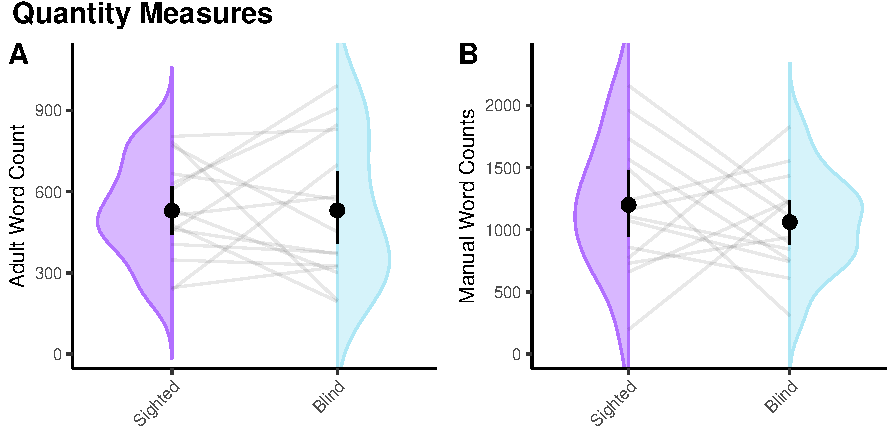
\includegraphics{input_quality_manuscript_files/figure-latex/quantity-plots-1} \caption{Comparing LENA-generated adult word counts (left) and transcription-based word counts in the input of blind and sighted children. Violin density represents the distribution of word counts for each group. Grey lines connect values from matched participants. Black dot and whiskers show standard error around the mean. Neither measure differed between groups.}\label{fig:quantity-plots}
\end{figure}

\hypertarget{interaction-1}{%
\subsubsection{Interaction}\label{interaction-1}}

Our corpus also revealed no significant difference in amount of interaction with the child, measured as the proportion of child-directed speech (\emph{t}(14) = 0.24, \emph{p} = .811) or in conversational turn counts to blind children versus to sighted children (\emph{W} = 61, \emph{p} = .978). Across both groups, child-directed speech constituted approximately 56\% of the input, and children were involved in roughly 34 conversational turns per hour; see Figure \ref{fig:interaction-plots}.

\begin{figure}[H!]
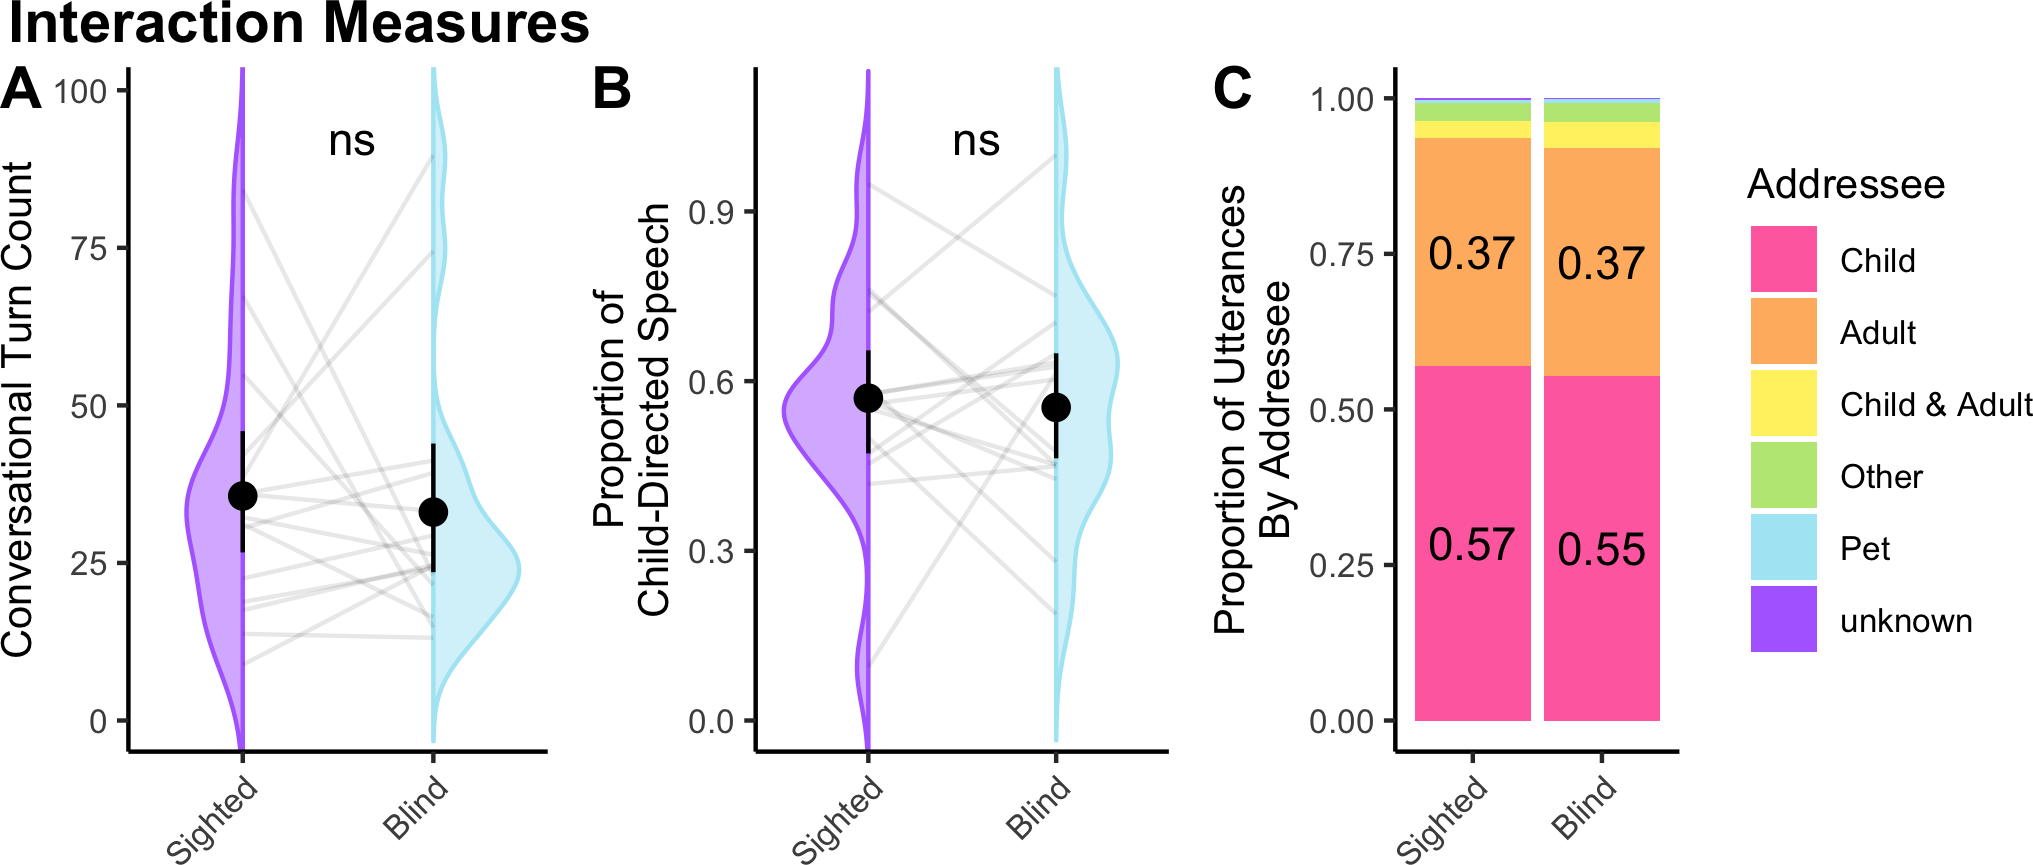
\includegraphics{input_quality_manuscript_files/figure-latex/interaction-plots-1} \caption{Comparing LENA-generated conversational turn counts (left) and proportion of utterances in child-directed speech (center).  Violin density represents the distribution of values for each group. Grey lines connect values from matched participants. Black dot and whiskers show standard error around the mean. The full breakdown by addressee is shown in the rightmost panel. Neither conversational turn count nor proportion of child-directed speech differed between groups.}\label{fig:interaction-plots}
\end{figure}

\hypertarget{linguistic-features-1}{%
\subsubsection{Linguistic Features}\label{linguistic-features-1}}

\begin{figure}[H!]
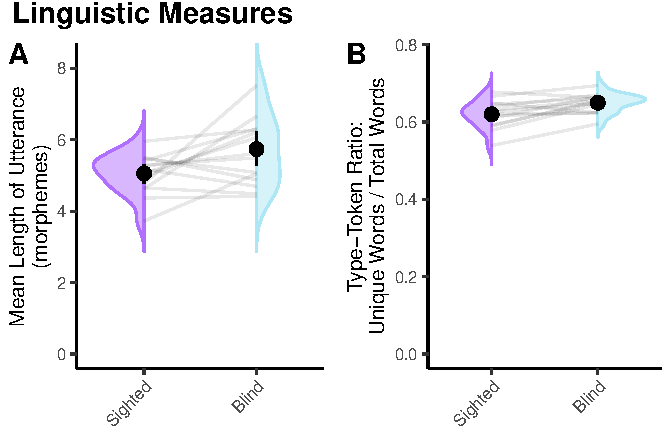
\includegraphics{input_quality_manuscript_files/figure-latex/linguistic-plots-1} \caption{Comparing linguistic features: Mean length of utterance (left) and type-token ratio (right). Violin density represents the distribution of values for each group. Grey lines connect values from matched participants. Black dot and whiskers show standard error around the mean. Utterances in blind children's input were significantly longer, and type-token ratio was significantly higher. Note that the y-axis on the type-token ratio plot has been truncated.}\label{fig:linguistic-plots}
\end{figure}

Similarly, neither linguistic variable differed across groups: blind and sighted children's input had comparable type-token ratios (\emph{t}(14) = -0.96, \emph{p} = .353) and utterance lengths (\emph{t}(14) = -2.02, \emph{p} = .063). Children in our samples hear on average 64 unique words per hundred words and 5.20 morphemes per utterance; see Figure \ref{fig:linguistic-plots}.

\hypertarget{conceptual-features-1}{%
\subsubsection{Conceptual Features}\label{conceptual-features-1}}

\begin{figure}[!H]
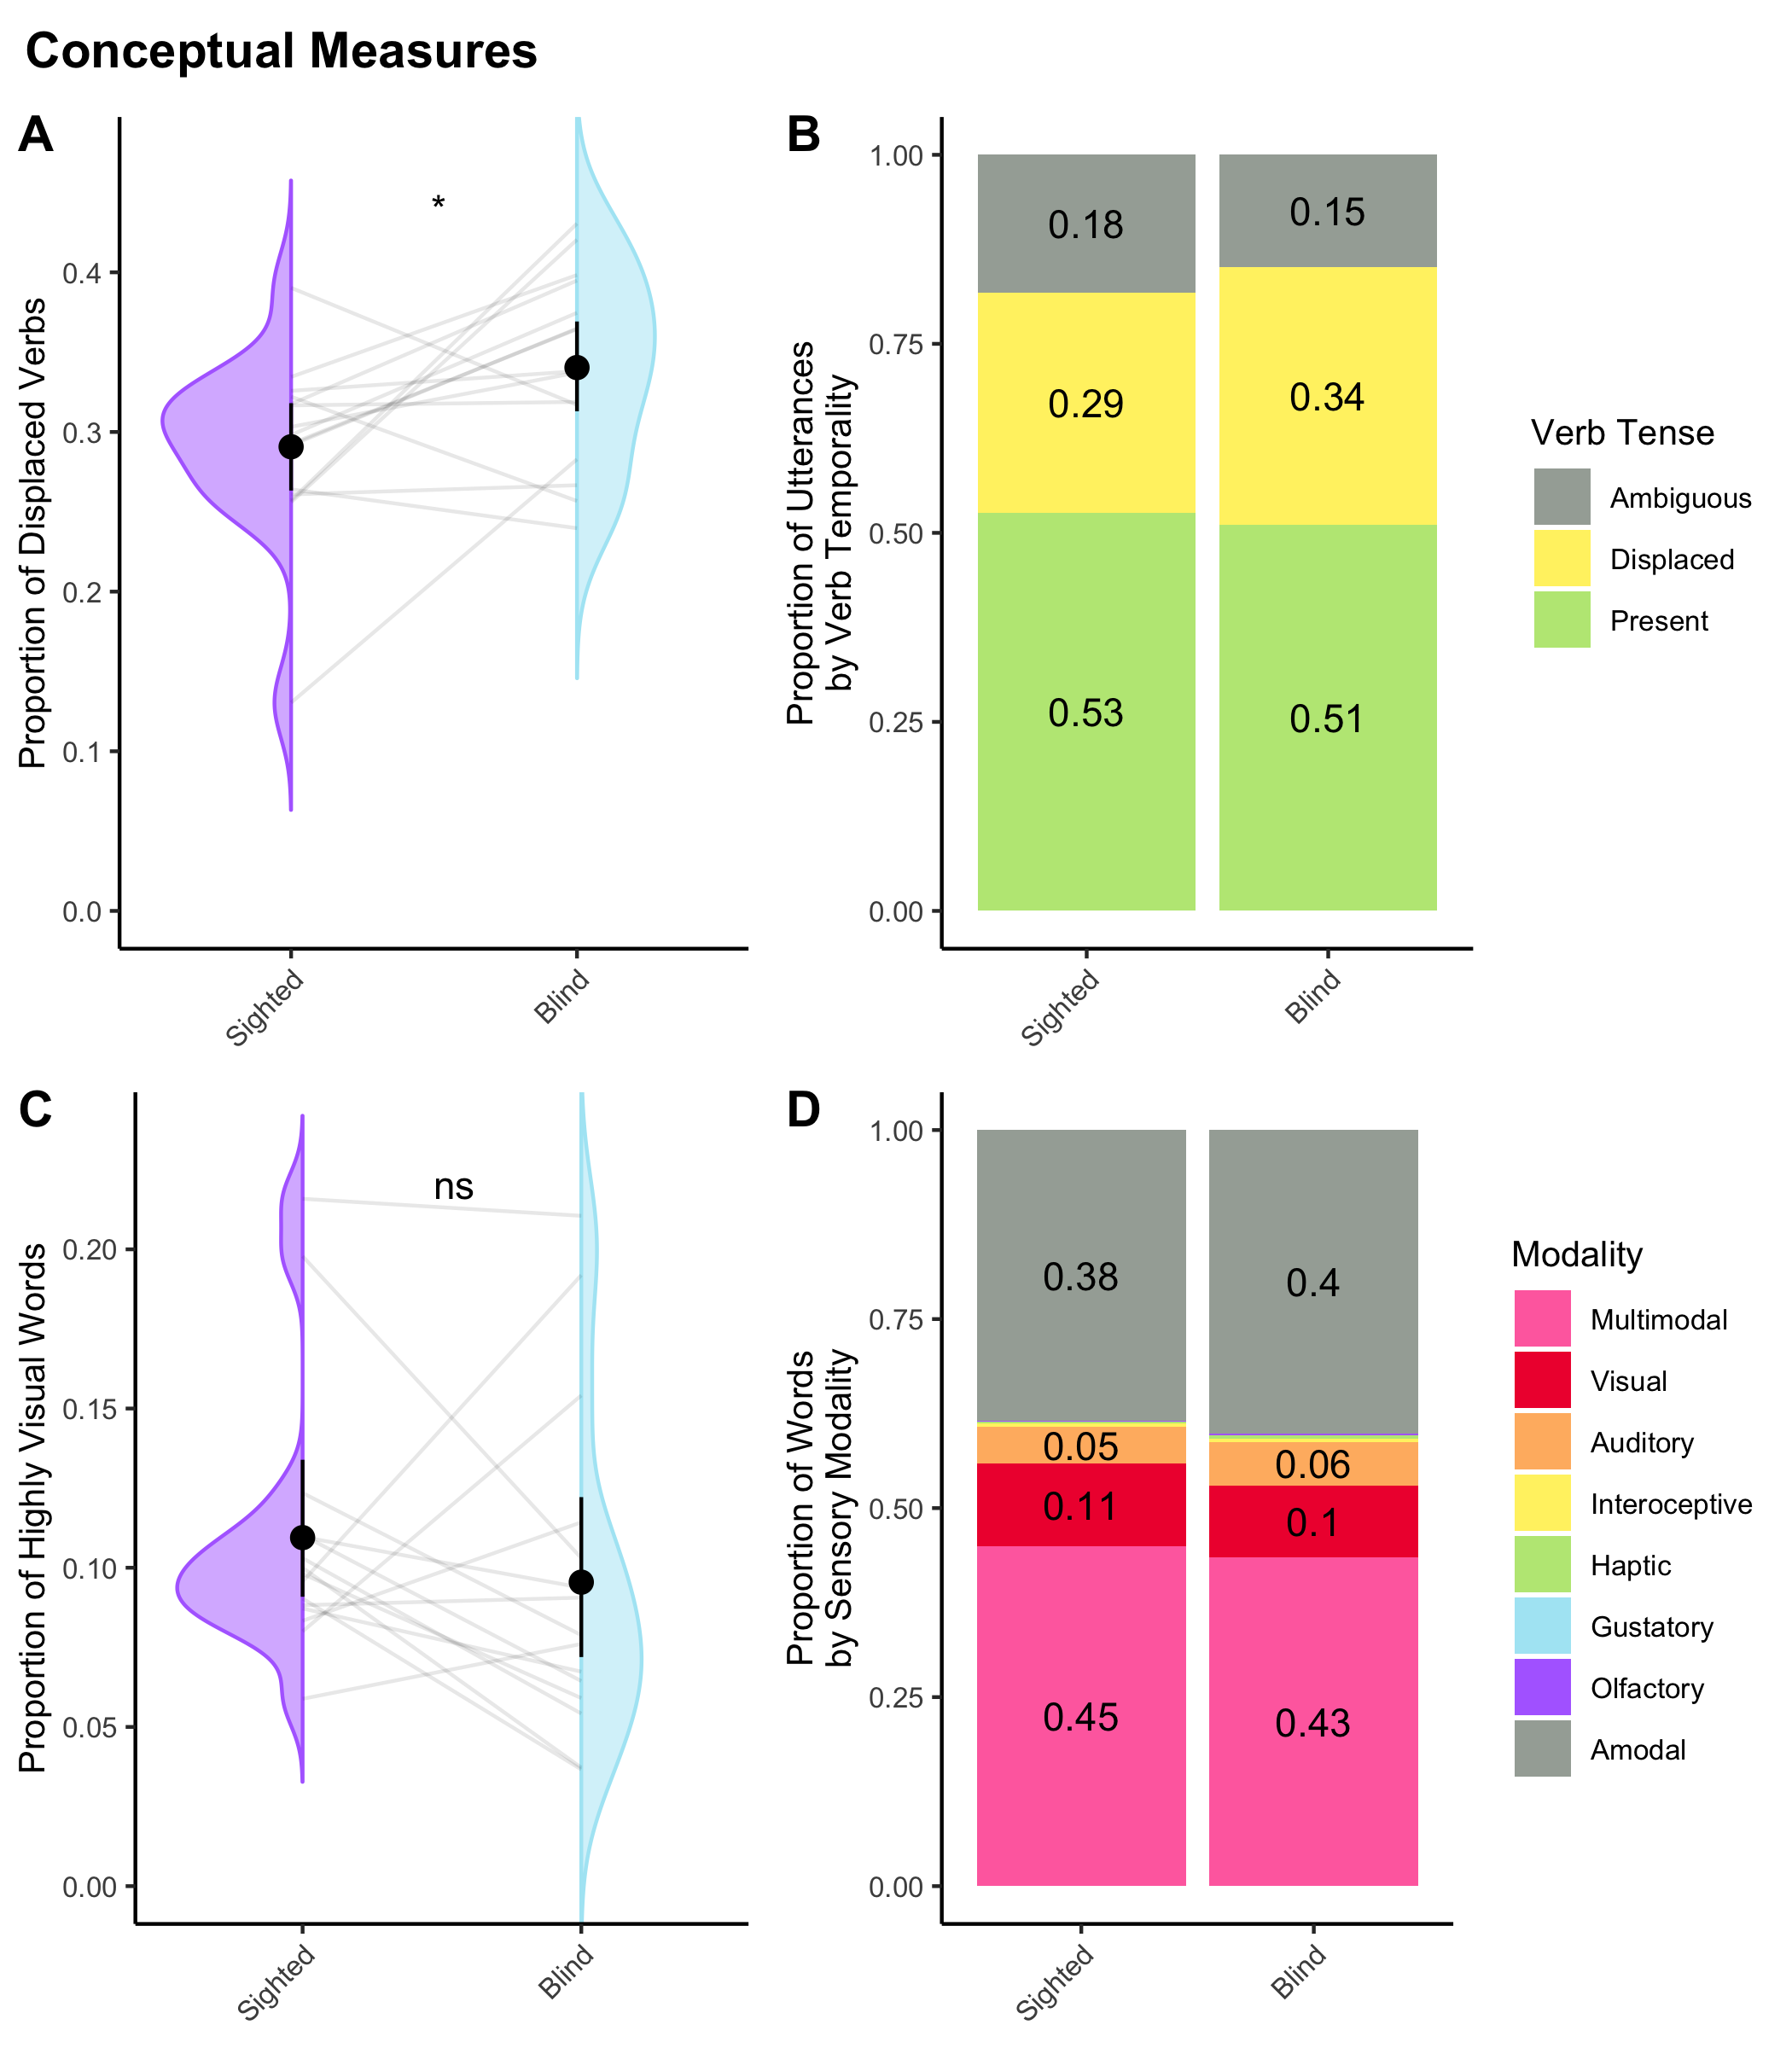
\includegraphics{input_quality_manuscript_files/figure-latex/conceptual-plots-1} \caption{Left col: Comparing proportion of temporally displaced verbs (top) and proportion of highly visual words (bottom). Violin density represents the distribution of values for each group. Grey lines connect values from matched participants. Black dot and whiskers show standard error around the mean. Right col: Full distribution of verb types (top)  and sensory modality (bottom) by group, collapsing across participants. Blind children's input contained significantly more temporally displaced verbs. Notably, the groups did not differ in the proportion of highly visual words.}\label{fig:conceptual-plots}
\end{figure}

Lastly, we compared two measures of the conceptual features of language input: the proportion of temporally displaced verbs and the proportion of highly visual words; see Figure \ref{fig:conceptual-plots}. We found that blind children hear a higher proportion of displaced verbs than sighted children (\emph{t}(14) = -2.68, \emph{p} = .018), which on average equates to 22 more utterances about past, future, or hypothetical events per hour. We found no significant difference across groups in the proportion of highly visual words (\emph{W} = 75, \emph{p} = .421), which constitute roughly 10\% of the input for both groups.

\begin{table}

\caption{\label{tab:analysis-summary-table}Summary of language input variables: how the measure is calculated; what portion of the recording the measure was calculated over; whether a parametric or non-parametric test was used; the mean, median, and range for blind and sighted children, and the raw (uncorrected) p-value of the test comparing groups. Only prop. displaced reached significance at our corrected p<.025 threshold for significance.}
\centering
\fontsize{9}{11}\selectfont
\begin{tabular}[t]{>{\raggedright\arraybackslash}p{.82in}|>{\raggedright\arraybackslash}p{2in}|>{\raggedright\arraybackslash}p{.76in}|>{\raggedright\arraybackslash}p{.6in}|>{\raggedright\arraybackslash}p{.7in}|>{\raggedright\arraybackslash}p{.8in}|>{\centering\arraybackslash}p{.43in}}
\hline
Variable & Description & Portion of Recording & Test & Blind Mean, Median, Range & Sighted Mean, Median, Range & p value\\
\hline
Adult Word Count & Estimated number of words in recording categorized as nearby adult speech by LENA algorithm & Whole day & t-test & 2124, 1808, 779-3968 words/hour & 2117, 2047, 951-3216 words/hour & .984\\
\hline
Manual Word Count & Number of word tokens from speakers other than target child & Random & t-test & 3994, 3504, 1208-7288 words/hour & 4598, 4296, 780-8668 words/hour & .307\\
\hline
Conversational Turn Count & Count of temporally close switches between adult and target-child vocalizations, divided by recording length & Whole day & Wilcoxon test & 66, 49, 26-180 turns/hour & 71, 65, 18-169 turns/hour & .811\\
\hline
Prop. Child-Directed Speech & Number of utterances tagged with child addressee out of total number of utterances, from speakers other than target child & Random & t-test & 0.55, 0.6, 0.19-1 & 0.57, 0.57, 0.09-0.95 & .978\\
\hline
Type-Token Ratio & Average of the type-token ratios (number of unique words divided by number of total words) for each of the 100-word bins in their sample & Random + High Volume & t-test & 0.64, 0.65, 0.58-0.67 unique words/ 100 words & 0.63, 0.63, 0.54-0.69 unique words/ 100 words & .353\\
\hline
Mean Length of Utterance & Average number of morphemes per utterance & Random + High Volume & t-test & 5.53, 5.28, 4.13-7.71 morphemes & 4.97, 5.11, 4.09-5.87 morphemes & .063\\
\hline
Prop. Displaced & Proportion of verbs that refer to past, future, or hypothetical events & Random + High Volume & t-test & 0.34, 0.33, 0.24-0.43 & 0.29, 0.3, 0.13-0.39 & .018*\\
\hline
Prop. Visual & Proportion of words in the input with high visual association ratings and low ratings for other perceptual modalities & Random + High Volume & Wilcoxon test & 0.1, 0.08, 0.04-0.21 & 0.11, 0.1, 0.06-0.22 & .421\\
\hline
\end{tabular}
\end{table}

\hypertarget{discussion}{%
\section{Discussion}\label{discussion}}

In this study, we analyzed the everyday language input to 15 young congenitally-blind children alongside a carefully peer-matched sighted sample using LENA audio recorders. While still relatively modest in absolute terms, this is a larger and more naturalistic sample than has previously been leveraged by prior work with this low-incidence population. We found that along the quantity, interaction, and linguistic dimensions, caregivers talked similarly to blind and sighted children, with small but potentially notable differences in conceptual content of the input. We discuss each of these results further below.

\hypertarget{quantity-1}{%
\subsection{Quantity}\label{quantity-1}}

Across two measures of language input quantity, one estimated from the full sixteen hour recording (Adult Word Count) and one precisely measured from a 30-minute samples from the day (Manual Word Count), blind and sighted children were exposed to similar amounts of speech in the home. Quantity was highly variable \emph{within} groups, but we found no evidence for \emph{between} group differences in input quantity. This runs counter to two folk accounts of language input to blind children: 1) that sighted parents of blind children might talk \emph{less} because they don't share visual common ground with their children; 2) that parents of blind children might talk \emph{more} to compensate for their children's lack of visual input. Instead, we find a similar quantity of speech across groups.

\hypertarget{interaction-2}{%
\subsection{Interaction}\label{interaction-2}}

We quantified interaction in two ways: through the LENA-estimated conversational turn count and through the proportion of child-directed speech in our manual annotations. Again, we found no differences across groups in the amount of parent-child interaction. This finding contrasts with previous research; other studies report \emph{less} interaction in dyads where the child is blind (Andersen et al., 1993; Grumi et al., 2021; Kekelis \& Andersen, 1984; Moore \& McConachie, 1994; Pérez-Pereira \& Conti-Ramsden, 2001; Preisler, 1991; Charity Rowland, 1984). Using a non-visual sampling method (i.e., our audio recordings) might provide a different, more naturalistic perspective on parent-child interactions, particularly in this population. For one thing, many prior studies (e.g., Kekelis \& Andersen, 1984; Moore \& McConachie, 1994; Pérez-Pereira \& Conti-Ramsden, 2001; Preisler, 1991) involve videorecordings in the child's home, with the researcher present. Like other young children, blind children distinguish between familiar individuals and strangers, and react with trepidation to the presence of a stranger; for blind children, this reaction may involve ``quieting'', wherein children cease speaking or vocalizing when they hear a new voice in the home (Fraiberg, 1975; McRae, 2002). By having a researcher present during the recordings\footnote{Fraiberg (1975) writes ``these fear and avoidance behaviors appear even though the observer, a twice-monthly visitor, is not, strictly speaking, a stranger.'' (pg. 323).}, prior research may have artificially suppressed blind children's initiation of interactions. Even naturalistic, observer-free videorecordings appear to inflate aspects of parental input, relative to daylong audio recordings (Bergelson et al., 2019). Together, these factors could explain why past parent-child interaction research finds that blind children initiate fewer interactions (Andersen et al., 1993; Dote-Kwan, 1995; Kekelis \& Andersen, 1984; Moore \& McConachie, 1994; Tröster \& Brambring, 1992), that parents do most of the talking (Andersen et al., 1993; Kekelis \& Andersen, 1984), and that there is overall less interaction (Nagayoshi et al., 2017; Rogers \& Puchalski, 1984; Charity Rowland, 1984; Tröster \& Brambring, 1992).

Additionally, a common focus in earlier interaction literature is to measure visual cues of interaction, such as shared gaze or attentiveness to facial expressions (Baird, Mayfield, \& Baker, 1997; Preisler, 1991; Rogers \& Puchalski, 1984). We can't help but wonder: are visual markers of social interaction the right yardstick to measure blind children against? In line with MacLeod and Demers (2023), perhaps the field should move away from sighted indicators of interaction ``quality'', and instead situate blind children's interactions within their own developmental niche, one that may be better captured with auditory- or tactile-focused measures.

\hypertarget{linguistic-features-2}{%
\subsection{Linguistic Features}\label{linguistic-features-2}}

Along the linguistic dimension, we measured type-token ratio and mean length of utterance. Parents of children with disabilities (including parents of blind children, e.g., Chernyak, n.d.; FamilyConnect, n.d.) are often advised to use shorter, simpler sentences with their children; correspondingly, previous work finds that parents of children with disabilities tend to find that parents \emph{do} use shorter, simpler utterances (e.g., Down syndrome, Lorang et al., 2020; hearing loss, Dirks et al., 2020). We therefore expected to observe shorter utterances and less lexical diversity in speech to blind vs.~sighted children. Instead, we found that blind children heard indistinguishable input by these metrics, with, if anything, a (marginally significant) trend towards \emph{longer} sentences in their input (relative to sighted matches, roughly half a word longer on average). Returning to the potential impact of input properties on children, evidence suggests that (contrary to the advice often given to parents), longer, more complex utterances are associated with better child language outcomes in both typically-developing children (Hoff \& Naigles, 2002) and children with cognitive differences (Sandbank \& Yoder, 2016). And similarly, higher lexical diversity is associated with larger vocabulary (Anderson et al., 2021; Hsu et al., 2017; Huttenlocher et al., 2010; Rowe, 2012; Weizman \& Snow, 2001). Regardless, the present analysis did not reveal robust statistical evidence that, at least on the group level, caregivers systematically provide utterances with different length or lexical diversity as a function of whether their child could see.

\hypertarget{conceptual-features-2}{%
\subsection{Conceptual Features}\label{conceptual-features-2}}

Although there are many potential ways to measure the conceptual features of language, we chose to capture \emph{here-and-now}-ness by measuring the proportion of temporally displaced verbs and the proportion of highly visual words. We found that blind children heard roughly 5\% more temporally displaced verbs than sighted peers. Moreover, though blind and sighted participants were exposed to a similar proportion of highly visual words, the referents of these words are by definition, inaccessible to the blind participants. Taken together, our conceptual results suggest that blind children's input is \emph{less} focused on the \emph{here-and-now}.

The extent to which blind children's language input is centered on the \emph{here-and-now} has been contested in the literature (Andersen et al., 1993; J. Campbell, 2003; Kekelis \& Andersen, 1984; Moore \& McConachie, 1994; Urwin, 1984). This aspect of language input is of particular interest because early reports suggest that blind children's own use of decontextualized language develops later than sighted children's (Bigelow, 1990; Urwin, 1984). Could such a difference be attributable to an absence of decontextualized language in the input? Our results suggest this is unlikely: we find that blind children's input contains \emph{more} decontextualized language rather than less. Speculatively, this may be because blind children have less access to immediate visual cues, leading to caregivers more frequently referring to past or future events to engage with their child. To illustrate, while riding on a train, instead of describing the scenery passing outside the window, parents may choose to talk about what happened earlier in the day or their plans upon arriving home. Without further information about the social and perceptual context, it is difficult to determine the communicative function of the differences we find in conceptual features we find or how they might explain differences in children's decontextualized language use. As more dense annotation becomes available, we look forward to further work exploring the social and environmental contexts of conceptual information as it unfolds across discourse.

It is worth underscoring again how much variability there is \emph{within} groups and how much consistency there is \emph{between} groups. One could imagine a world in which the language environments of blind and sighted children are radically different from each other. Our data do not support that hypothesis. Rather, we find similarity in quantity, interaction, and linguistic properties, alongside modest differences in conceptual properties. That is, in line with recent work highlighting immense \emph{within}-group variability across many different socio-cultural and linguistic contexts (Bergelson et al., 2023), our blind and sighted groups here have large within-group variability but very few between-group differences. Despite strikingly different visual experiences, young blind and sighted learners have at best modest differences in their speech environments.

\hypertarget{connecting-to-language-outcomes}{%
\subsection{Connecting to Language Outcomes}\label{connecting-to-language-outcomes}}

Our results uncover no systematic group differences in the quantity of speech, amount of language interaction, or linguistic complexity parents provide to blind vs.~sighted children, at least as measured here. When we do see differences, language input to blind children looks more conceptually complex or perceptually unavailable. In other populations, complexity of this sort is linked with \emph{more} sophisticated child language outcomes (Demir et al., 2015; Rowe, 2012; Uccelli et al., 2019), so it is not the case that blind children's language input is ``impoverished'' in this sense.

In our modestly-sized, predominantly pre-lexical sample, linking language input to children's language outcomes directly is not yet feasible, but prior literature allows us to speculate on two possibilities. First, if input effects pattern similarly for blind and sighted children, we would expect blind and sighted children alike to benefit from more input (Anderson et al., 2021; Gilkerson et al., 2018; Huttenlocher et al., 1991; Rowe, 2008), more interactive input (Donnellan et al., 2020; Goldstein \& Schwade, 2008; Hirsh-Pasek et al., 2015; Romeo et al., 2018; Rowe, 2008; Shneidman et al., 2013; Weisleder \& Fernald, 2013), more linguistically complex input (Anderson et al., 2021; De Villiers, 1985; Hadley et al., 2017; Hoff, 2003; Hsu et al., 2017; Huttenlocher et al., 2002, 2010; Naigles \& Hoff-Ginsberg, 1998; Rowe, 2012; Weizman \& Snow, 2001), and more conceptually complex input (Demir et al., 2015; Rowe, 2012; Uccelli et al., 2019).

At the same time, however, recent results show that blind children have a roughly half-year delay in their productive vocabulary, relative to sighted peers (E. E. Campbell et al., 2024). If properties of the language input play a role in this delay, this raises the second possibility: that language input affects acquisition \emph{differently} for blind children than it does for sighted children. Under this possibility, blind children would benefit from \emph{less} complex language input, and the equivalencies in quantity, linguistic complexity and interactivity alongside the increased conceptual complexity we find here would, in theory, contribute to early vocabulary delays.

To show our cards, we are inclined towards option one: that blind children benefit from language input in the same ways as sighted peers (Landau \& Gleitman, 1985), and that this additionally extends to the benefits of receiving more conceptually complex language input. Language regularly supports learning in the absence of direct sensory perception (e.g., reading a book about mythical creatures). Given the language skills of blind adults (Loiotile et al., 2020; Röder et al., 2003; Röder et al., 2000), it is undeniable that language is a rich source of meaning for blind individuals as well (E. E. Campbell \& Bergelson, 2022; Lewis, Zettersten, \& Lupyan, 2019; van Paridon, Liu, \& Lupyan, 2021). Testing each of these predictions--as well as whether links between language input and language outcomes change across developmental time--awaits further research.

In either case, if properties of language input do influence blind children's language outcomes, attempting to train parents to talk differently may be unfruitful. While some interventions where parents are trained to talk differently to their children show promise (Huber, Ferjan Ramírez, Corrigan, \& Kuhl, 2023; Roberts, Curtis, Sone, \& Hampton, 2019), such interventions often fail to change parental speech patterns on more extended timescales (e.g., McGillion, Pine, Herbert, \& Matthews, 2017; Suskind et al., 2016).

\hypertarget{conclusion}{%
\section{Conclusion}\label{conclusion}}

In summary, our study compared language input in homes of 15 blind and 15 sighted infants. We found that both groups received language input with similar quantities of speech, interactivity, and linguistic complexity. Additionally, blind children were exposed to input that had somewhat more conceptual complexity, in terms of discussion beyond the here-and-now and words for less perceptually-avaiable (visual) referents. This suggests that young blind children are being exposed to a rich linguistic environment that differs only modestly from the language input of sighted children. Our study does not imply that parents should change their communication styles, but rather highlights the language experiences of blind children. Future research linking input links to language development and cognitive abilities of blind and sighted children alike would be a fruitful and welcome next step.

\hypertarget{ethics}{%
\section{Ethics}\label{ethics}}

This study received approval from the Duke University Institutional Review Board. All families consented to take part in this research.

\hypertarget{data-code-and-materials-availability}{%
\section{Data, Code and Materials Availability}\label{data-code-and-materials-availability}}

LENA data, transcripts, and code for all analyses presented in this article are available on \href{https://osf.io/dcnq6/}{OSF}.

\hypertarget{authorship}{%
\section{Authorship}\label{authorship}}

\textbf{Erin Campbell:} Conceptualization, Validation, Investigation, Analysis, Data Curation, Writing - Original Draft, Writing - Review \& Editing, Visualization, Project Administration; \textbf{Lillianna Righter:} Validation, Analysis, Data Curation, Writing - Original Draft, Writing - Review \& Editing, Project Administration; \textbf{Eugenia Lukin:} Validation, Writing - Review \& Editing; \textbf{Elika Bergelson:} Conceptualization, Resources, Writing - Review \& Editing, Visualization, Supervision, Funding Acquisition

\hypertarget{acknowledgements}{%
\section{Acknowledgements}\label{acknowledgements}}

We wish to thank the following individuals who generously contributed recordings for the sighted matches: Anne Warlaumont, Derek Houston, Nairán Ramírez-Esparza, Mark VanDam, Caroline Rowland. We thank Zhenya Kalenkovich and Alex Emmert for careful code review.

\hypertarget{references}{%
\section*{References}\label{references}}
\addcontentsline{toc}{section}{References}

\hypertarget{refs}{}
\begin{CSLReferences}{1}{0}
\leavevmode\vadjust pre{\hypertarget{ref-abu-zhaya2019}{}}%
Abu-Zhaya, R., Kondaurova, M. V., Houston, D., \& Seidl, A. (2019). Vocal and {Tactile Input} to {Children Who Are Deaf} or {Hard} of {Hearing}. \emph{Journal of Speech, Language, and Hearing Research}, \emph{62}(7), 2372--2385. \url{https://doi.org/10.1044/2019_JSLHR-L-18-0185}

\leavevmode\vadjust pre{\hypertarget{ref-andersen1993}{}}%
Andersen, E. S., Dunlea, A., \& Kekelis, L. (1993). The impact of input: Language acquisition in the visually impaired. \emph{First Language}, \emph{13}(37), 23--49. \url{https://doi.org/10.1177/014272379301303703}

\leavevmode\vadjust pre{\hypertarget{ref-anderson2021}{}}%
Anderson, N. J., Graham, S. A., Prime, H., Jenkins, J. M., \& Madigan, S. (2021). Linking {Quality} and {Quantity} of {Parental Linguistic Input} to {Child Language Skills}: {A Meta-Analysis}. \emph{Child Development}, \emph{92}(2), 484--501. \url{https://doi.org/10.1111/cdev.13508}

\leavevmode\vadjust pre{\hypertarget{ref-baird1997}{}}%
Baird, S. M., Mayfield, P., \& Baker, P. (1997). Mothers' {Interpretations} of the {Behavior} of {Their Infants} with {Visual} and {Other Impairments} during {Interactions}. \emph{Journal of Visual Impairment \& Blindness}, \emph{91}(5), 467--483. \url{https://doi.org/10.1177/0145482X9709100507}

\leavevmode\vadjust pre{\hypertarget{ref-benjamini1995}{}}%
Benjamini, Y., \& Hochberg, Y. (1995). Controlling the {False Discovery Rate}: {A Practical} and {Powerful Approach} to {Multiple Testing}. \emph{Journal of the Royal Statistical Society. Series B (Methodological)}, \emph{57}(1), 289--300. Retrieved from \url{https://www.jstor.org/stable/2346101}

\leavevmode\vadjust pre{\hypertarget{ref-bergelson2015a}{}}%
Bergelson, E. (2015). \emph{Bergelson {Seedlings HomeBank Corpus}}. TalkBank. \url{https://doi.org/10.21415/T5PK6D}

\leavevmode\vadjust pre{\hypertarget{ref-bergelson2019}{}}%
Bergelson, E., Amatuni, A., Dailey, S., Koorathota, S., \& Tor, S. (2019). Day by day, hour by hour: {Naturalistic} language input to infants. \emph{Developmental Science}, \emph{22}(1), e12715. \url{https://doi.org/10.1111/desc.12715}

\leavevmode\vadjust pre{\hypertarget{ref-bergelson2023}{}}%
Bergelson, E., Soderstrom, M., Schwarz, I.-C., Rowland, C., Ramírez-Esparza, N., R. Hamrick, L., \ldots{} Cristia, A. (2023). Everyday language input and production in 1,001 children from six continents. \emph{Proceedings of the National Academy of Sciences}, \emph{120}(52), e2300671120. \url{https://doi.org/10.1073/pnas.2300671120}

\leavevmode\vadjust pre{\hypertarget{ref-bergelson2013}{}}%
Bergelson, E., \& Swingley, D. (2013). The acquisition of abstract words by young infants. \emph{Cognition}, \emph{127}(3), 391--397. \url{https://doi.org/10.1016/j.cognition.2013.02.011}

\leavevmode\vadjust pre{\hypertarget{ref-bernsteinratner1984}{}}%
Bernstein Ratner, N. (1984). Patterns of vowel modification in mother--child speech. \emph{Journal of Child Language}, \emph{11}, 557--578.

\leavevmode\vadjust pre{\hypertarget{ref-bigelow1987}{}}%
Bigelow, A. (1987). Early words of blind children. \emph{Journal of Child Language}, \emph{14}(1), 47--56. \url{https://doi.org/10.1017/S0305000900012721}

\leavevmode\vadjust pre{\hypertarget{ref-bigelow1990}{}}%
Bigelow, A. (1990). Relationship between the {Development} of {Language} and {Thought} in {Young Blind Children}. \emph{Journal of Visual Impairment \& Blindness}, \emph{84}(8), 414--419. \url{https://doi.org/10.1177/0145482X9008400805}

\leavevmode\vadjust pre{\hypertarget{ref-bratt2022}{}}%
Bratt, J., Harmon, J., \& Learning, B. F. \&. W. P. G. L. D. M. (2022). \emph{Morphemepiece: {Morpheme Tokenization}}.

\leavevmode\vadjust pre{\hypertarget{ref-brugman2009}{}}%
Brugman, H., \& Russel, A. (2009). Annotating {Multimedia} / {Multi-modal} resources with {ELAN}. \emph{Proceedings of the Fourth International Conference on Language Resources and Evaluation}.

\leavevmode\vadjust pre{\hypertarget{ref-busch2018}{}}%
Busch, T., Sangen, A., Vanpoucke, F., \& van Wieringen, A. (2018). Correlation and agreement between {Language ENvironment Analysis} ({LENA}™) and manual transcription for {Dutch} natural language recordings. \emph{Behavior Research Methods}, \emph{50}(5), 1921--1932. \url{https://doi.org/10.3758/s13428-017-0960-0}

\leavevmode\vadjust pre{\hypertarget{ref-campbell2022}{}}%
Campbell, E. E., \& Bergelson, E. (2022). Making sense of sensory language: {Acquisition} of sensory knowledge by individuals with congenital sensory impairments. \emph{Neuropsychologia}, \emph{174}, 108320. \url{https://doi.org/10.1016/j.neuropsychologia.2022.108320}

\leavevmode\vadjust pre{\hypertarget{ref-campbell2024}{}}%
Campbell, E. E., Casillas, R., \& Bergelson, E. (2024). The role of vision in the acquisition of words: {Vocabulary} development in blind toddlers. \emph{Developmental Science}, \emph{n/a}(n/a), e13475. \url{https://doi.org/10.1111/desc.13475}

\leavevmode\vadjust pre{\hypertarget{ref-campbell2003}{}}%
Campbell, J. (2003). Maternal {Directives} to {Young Children} who are {Blind}. \emph{Journal of Visual Impairment \& Blindness}, \emph{97}(6), 355--365. \url{https://doi.org/10.1177/0145482X0309700604}

\leavevmode\vadjust pre{\hypertarget{ref-casillas2020}{}}%
Casillas, M., Brown, P., \& Levinson, S. C. (2020). Early {Language Experience} in a {Tseltal Mayan Village}. \emph{Child Development}, \emph{91}(5), 1819--1835. \url{https://doi.org/10.1111/cdev.13349}

\leavevmode\vadjust pre{\hypertarget{ref-chernyak}{}}%
Chernyak, P. (n.d.). 3 {Ways} to {Teach Your Blind} or {Visually Impaired Child} to {Talk}. https://www.wikihow.life/Teach-Your-Blind-or-Visually-Impaired-Child-to-Talk.

\leavevmode\vadjust pre{\hypertarget{ref-chiesa2015}{}}%
Chiesa, S., Galati, D., \& Schmidt, S. (2015). Communicative interactions between visually impaired mothers and their sighted children: Analysis of gaze, facial expressions, voice and physical contacts. \emph{Child: Care, Health and Development}, \emph{41}(6), 1040--1046. \url{https://doi.org/10.1111/cch.12274}

\leavevmode\vadjust pre{\hypertarget{ref-cristia2020}{}}%
Cristia, A., Bulgarelli, F., \& Bergelson, E. (2020). Accuracy of the {Language Environment Analysis System Segmentation} and {Metrics}: {A Systematic Review}. \emph{Journal of Speech, Language, and Hearing Research}, \emph{63}(4), 1093--1105. \url{https://doi.org/10.1044/2020_JSLHR-19-00017}

\leavevmode\vadjust pre{\hypertarget{ref-devilliers1985}{}}%
De Villiers, J. (1985). Learning how to use verbs: Lexical coding and the influence of the input*. \emph{Journal of Child Language}, \emph{12}(3), 587--595. \url{https://doi.org/10.1017/S0305000900006668}

\leavevmode\vadjust pre{\hypertarget{ref-demir2015}{}}%
Demir, Ö. E., Rowe, M. L., Heller, G., Goldin-Meadow, S., \& Levine, S. C. (2015). Vocabulary, syntax, and narrative development in typically developing children and children with early unilateral brain injury: Early parental talk about the "there-and-then" matters. \emph{Developmental Psychology}, \emph{51}(2), 161--175. \url{https://doi.org/10.1037/a0038476}

\leavevmode\vadjust pre{\hypertarget{ref-dirks2020}{}}%
Dirks, E., Stevens, A., Kok, S., Frijns, J., \& Rieffe, C. (2020). Talk with me! {Parental} linguistic input to toddlers with moderate hearing loss. \emph{Journal of Child Language}, \emph{47}(1), 186--204. \url{https://doi.org/10.1017/S0305000919000667}

\leavevmode\vadjust pre{\hypertarget{ref-donnellan2020}{}}%
Donnellan, E., Bannard, C., McGillion, M. L., Slocombe, K. E., \& Matthews, D. (2020). Infants' intentionally communicative vocalizations elicit responses from caregivers and are the best predictors of the transition to language: {A} longitudinal investigation of infants' vocalizations, gestures and word production. \emph{Developmental Science}, \emph{23}(1), e12843. \url{https://doi.org/10.1111/desc.12843}

\leavevmode\vadjust pre{\hypertarget{ref-dote-kwan1995}{}}%
Dote-Kwan, J. (1995). Impact of {Mothers}' {Interactions} on the {Development} of {Their Young Visually Impaired Children}. \emph{Journal of Visual Impairment \& Blindness}, \emph{89}(1), 46--58. \url{https://doi.org/10.1177/0145482X9508900109}

\leavevmode\vadjust pre{\hypertarget{ref-familyconnect}{}}%
FamilyConnect. (n.d.). Understanding the {Stages} of {Language Development} for {Babies Who Are Blind}.

\leavevmode\vadjust pre{\hypertarget{ref-fenson1994}{}}%
Fenson, L., Dale, P. S., Reznick, J. S., Bates, E., Thal, D. J., Pethick, S. J., \ldots{} Stiles, J. (1994). Variability in {Early Communicative Development}. \emph{Monographs of the Society for Research in Child Development}, \emph{59}(5), i. \url{https://doi.org/10.2307/1166093}

\leavevmode\vadjust pre{\hypertarget{ref-ferjanramirez2021}{}}%
Ferjan Ramírez, N., Hippe, D. S., \& Kuhl, P. K. (2021). Comparing {Automatic} and {Manual Measures} of {Parent}--{Infant Conversational Turns}: {A Word} of {Caution}. \emph{Child Development}, \emph{92}(2), 672--681. \url{https://doi.org/10.1111/cdev.13495}

\leavevmode\vadjust pre{\hypertarget{ref-fernald1989}{}}%
Fernald, A. (1989). \href{https://www.ncbi.nlm.nih.gov/pubmed/2612255}{Intonation and communicative intent in mothers' speech to infants: Is the melody the message?} \emph{Child Development}, \emph{60}(6), 1497--1510.

\leavevmode\vadjust pre{\hypertarget{ref-fernald1993}{}}%
Fernald, A., \& Morikawa, H. (1993). \href{https://www.ncbi.nlm.nih.gov/pubmed/8339686}{Common themes and cultural variations in {Japanese} and {American} mothers' speech to infants}. \emph{Child Development}, \emph{64}(3), 637--656.

\leavevmode\vadjust pre{\hypertarget{ref-fraiberg1975}{}}%
Fraiberg, S. (1975). The development of human attachments in infants blind from birth. \emph{Merrill-Palmer Quarterly}, \emph{21}, 315--334.

\leavevmode\vadjust pre{\hypertarget{ref-ganea2018}{}}%
Ganea, N., Hudry, K., Vernetti, A., Tucker, L., Charman, T., Johnson, M. H., \& Senju, A. (2018). Development of adaptive communication skills in infants of blind parents. \emph{Developmental Psychology}, \emph{54}(12), 2265--2273. \url{https://doi.org/10.1037/dev0000564}

\leavevmode\vadjust pre{\hypertarget{ref-ganek2016}{}}%
Ganek, H., \& Eriks-Brophy, A. (2016). The {Language ENvironment Analysis} ({LENA}) system: {A} literature review. \emph{Proceedings of the Joint Workshop on {NLP} for {Computer Assisted Language Learning} and {NLP} for {Language Acquisition}}, 24--32. Ume{å}, Sweden: LiU Electronic Press.

\leavevmode\vadjust pre{\hypertarget{ref-ganek2018}{}}%
Ganek, H., \& Eriks-Brophy, A. (2018). Language {ENvironment} analysis ({LENA}) system investigation of day long recordings in children: {A} literature review. \emph{Journal of Communication Disorders}, \emph{72}, 77--85. \url{https://doi.org/10.1016/j.jcomdis.2017.12.005}

\leavevmode\vadjust pre{\hypertarget{ref-gergle2004}{}}%
Gergle, D., Kraut, R. E., \& Fussell, S. R. (2004). Language {Efficiency} and {Visual Technology}: {Minimizing Collaborative Effort} with {Visual Information}. \emph{Journal of Language and Social Psychology}, \emph{23}(4), 491--517. \url{https://doi.org/10.1177/0261927X04269589}

\leavevmode\vadjust pre{\hypertarget{ref-gilkerson2008}{}}%
Gilkerson, J., \& Richards, J. A. (2008). \emph{The {LENA Natural Language Study}}. Boulder, CO: LENA Foundation.

\leavevmode\vadjust pre{\hypertarget{ref-gilkerson2018}{}}%
Gilkerson, J., Richards, J. A., Warren, S. F., Oller, D. K., Russo, R., \& Vohr, B. (2018). Language {Experience} in the {Second Year} of {Life} and {Language Outcomes} in {Late Childhood}. \emph{Pediatrics}, \emph{142}(4), e20174276. \url{https://doi.org/10.1542/peds.2017-4276}

\leavevmode\vadjust pre{\hypertarget{ref-gleitman1990}{}}%
Gleitman, L. R. (1990). The {Structural Sources} of {Verb Meanings}. \emph{Language Acquisition}, \emph{1}(1), 3--55. Retrieved from \url{https://www.jstor.org/stable/20011341}

\leavevmode\vadjust pre{\hypertarget{ref-gleitman1995}{}}%
Gleitman, L. R., \& Newport, E. L. (1995). The invention of language by children: {Environmental} and biological influences on the acquisition of language. In \emph{An Invitation to Cognitive Science}. \emph{Language: {An} invitation to cognitive science, {Vol}. 1, 2nd ed} (pp. 1--24). Cambridge, MA, US: The MIT Press.

\leavevmode\vadjust pre{\hypertarget{ref-goldstein2008}{}}%
Goldstein, M. H., \& Schwade, J. A. (2008). Social feedback to infants' babbling facilitates rapid phonological learning. \emph{Psychological Science}, \emph{19}(5), 515--523. \url{https://doi.org/10.1111/j.1467-9280.2008.02117.x}

\leavevmode\vadjust pre{\hypertarget{ref-grice1975}{}}%
Grice, H. P. (1975). {Logic and Conversation}. In \emph{{Syntax and semantics}}. New York San Francisco London: Academic press, Harcourt Brace Jovanovich.

\leavevmode\vadjust pre{\hypertarget{ref-grigoroglou2016}{}}%
Grigoroglou, M., Edu, U., \& Papafragou, A. (2016). Are children flexible speakers? {Effects} of typicality and listener needs in children's event descriptions. \emph{Cognitive Science}, 6.

\leavevmode\vadjust pre{\hypertarget{ref-grimminger2020}{}}%
Grimminger, A., Rohlfing, K. J., Lüke, C., Liszkowski, U., \& Ritterfeld, U. (2020). Decontextualized talk in caregivers' input to 12-month-old children during structured interaction. \emph{Journal of Child Language}, \emph{47}(2), 418--434. \url{https://doi.org/10.1017/S0305000919000710}

\leavevmode\vadjust pre{\hypertarget{ref-grumi2021}{}}%
Grumi, S., Cappagli, G., Aprile, G., Mascherpa, E., Gori, M., Provenzi, L., \& Signorini, S. (2021). Togetherness, beyond the eyes: {A} systematic review on the interaction between visually impaired children and their parents. \emph{Infant Behavior and Development}, \emph{64}, 101590. \url{https://doi.org/10.1016/j.infbeh.2021.101590}

\leavevmode\vadjust pre{\hypertarget{ref-hadley2017}{}}%
Hadley, P. A., Rispoli, M., Holt, J. K., Papastratakos, T., Hsu, N., Kubalanza, M., \& McKenna, M. M. (2017). Input {Subject Diversity Enhances Early Grammatical Growth}: {Evidence} from a {Parent-Implemented Intervention}. \emph{Language Learning and Development: The Official Journal of the Society for Language Development}, \emph{13}(1), 54--79. \url{https://doi.org/10.1080/15475441.2016.1193020}

\leavevmode\vadjust pre{\hypertarget{ref-hawkins2021}{}}%
Hawkins, R. D., Gweon, H., \& Goodman, N. D. (2021). The {Division} of {Labor} in {Communication}: {Speakers Help Listeners Account} for {Asymmetries} in {Visual Perspective}. \emph{Cognitive Science}, \emph{45}(3), e12926. \url{https://doi.org/10.1111/cogs.12926}

\leavevmode\vadjust pre{\hypertarget{ref-hazan2011}{}}%
Hazan, V., \& Baker, R. (2011). Acoustic-phonetic characteristics of speech produced with communicative intent to counter adverse listening conditions. \emph{The Journal of the Acoustical Society of America}, \emph{130}(4), 2139--2152. \url{https://doi.org/10.1121/1.3623753}

\leavevmode\vadjust pre{\hypertarget{ref-hirsh-pasek2015}{}}%
Hirsh-Pasek, K., Adamson, L. B., Bakeman, R., Owen, M. T., Golinkoff, R. M., Pace, A., \ldots{} Suma, K. (2015). The {Contribution} of {Early Communication Quality} to {Low-Income Children}'s {Language Success}. \emph{Psychological Science}, \emph{26}(7), 1071--1083. \url{https://doi.org/10.1177/0956797615581493}

\leavevmode\vadjust pre{\hypertarget{ref-hoff2003}{}}%
Hoff, E. (2003). The specificity of environmental influence: Socioeconomic status affects early vocabulary development via maternal speech. \emph{Child Development}, \emph{74}(5), 1368--1378. \url{https://doi.org/10.1111/1467-8624.00612}

\leavevmode\vadjust pre{\hypertarget{ref-hoff2002}{}}%
Hoff, E., \& Naigles, L. (2002). How children use input to acquire a lexicon. \emph{Child Development}, \emph{73}(2), 418--433. \url{https://doi.org/10.1111/1467-8624.00415}

\leavevmode\vadjust pre{\hypertarget{ref-hsu2017}{}}%
Hsu, N., Hadley, P. A., \& Rispoli, M. (2017). Diversity matters: Parent input predicts toddler verb production. \emph{Journal of Child Language}, \emph{44}(1), 63--86. \url{https://doi.org/10.1017/S0305000915000690}

\leavevmode\vadjust pre{\hypertarget{ref-huber2023}{}}%
Huber, E., Ferjan Ramírez, N., Corrigan, N. M., \& Kuhl, P. K. (2023). Parent coaching from 6 to 18 months improves child language outcomes through 30 months of age. \emph{Developmental Science}, \emph{26}(6), e13391. \url{https://doi.org/10.1111/desc.13391}

\leavevmode\vadjust pre{\hypertarget{ref-hudson2002}{}}%
Hudson, J. A. (2002). "{Do You Know What We}'re {Going} to {Do This Summer}?": {Mothers}' {Talk} to {Preschool Children About Future Events}. \emph{Journal of Cognition and Development}, \emph{3}(1), 49--71. \url{https://doi.org/10.1207/S15327647JCD0301_4}

\leavevmode\vadjust pre{\hypertarget{ref-huttenlocher1991}{}}%
Huttenlocher, J., Haight, W., Bryk, A., Seltzer, M., \& Lyons, T. (1991). Early vocabulary growth: {Relation} to language input and gender. \emph{Developmental Psychology}, \emph{27}, 236--248. \url{https://doi.org/10.1037/0012-1649.27.2.236}

\leavevmode\vadjust pre{\hypertarget{ref-huttenlocher2002}{}}%
Huttenlocher, J., Vasilyeva, M., Cymerman, E., \& Levine, S. (2002). Language input and child syntax. \emph{Cognitive Psychology}, \emph{45}(3), 337--374. \url{https://doi.org/10.1016/s0010-0285(02)00500-5}

\leavevmode\vadjust pre{\hypertarget{ref-huttenlocher2010}{}}%
Huttenlocher, J., Waterfall, H., Vasilyeva, M., Vevea, J., \& Hedges, L. V. (2010). Sources of variability in children's language growth. \emph{Cognitive Psychology}, \emph{61}(4), 343--365. \url{https://doi.org/10.1016/j.cogpsych.2010.08.002}

\leavevmode\vadjust pre{\hypertarget{ref-jara-ettinger2021}{}}%
Jara-Ettinger, J., \& Rubio-Fernandez, P. (2021). The social basis of referential communication: {Speakers} construct physical reference based on listeners' expected visual search. \emph{Psychological Review}, No Pagination Specified--No Pagination Specified. \url{https://doi.org/10.1037/rev0000345}

\leavevmode\vadjust pre{\hypertarget{ref-kekelis1984}{}}%
Kekelis, L. S., \& Andersen, E. S. (1984). Family {Communication Styles} and {Language Development}. \emph{Journal of Visual Impairment \& Blindness}, \emph{78}(2), 54--65. \url{https://doi.org/10.1177/0145482X8407800202}

\leavevmode\vadjust pre{\hypertarget{ref-kramer1975}{}}%
Kramer, J. A., Hill, K. T., \& Cohen, L. B. (1975). Infants' {Development} of {Object Permanence}: {A Refined Methodology} and {New Evidence} for {Piaget}'s {Hypothesized Ordinality}. \emph{Child Development}, \emph{46}(1), 149--155. \url{https://doi.org/10.2307/1128843}

\leavevmode\vadjust pre{\hypertarget{ref-landau1985}{}}%
Landau, B., \& Gleitman, L. R. (1985). \emph{Language and experience: {Evidence} from the blind child} (pp. xi, 250). Cambridge, MA, US: Harvard University Press.

\leavevmode\vadjust pre{\hypertarget{ref-lavechin2021}{}}%
Lavechin, M., Bousbib, R., Bredin, H., Dupoux, E., \& Cristia, A. (2021). \emph{An open-source voice type classifier for child-centered daylong recordings}. arXiv. \url{https://doi.org/10.48550/arXiv.2005.12656}

\leavevmode\vadjust pre{\hypertarget{ref-lehet2021}{}}%
Lehet, M., Arjmandi, M. K., Houston, D., \& Dilley, L. (2021). Circumspection in using automated measures: {Talker} gender and addressee affect error rates for adult speech detection in the {Language ENvironment Analysis} ({LENA}) system. \emph{Behavior Research Methods}, \emph{53}(1), 113--138. \url{https://doi.org/10.3758/s13428-020-01419-y}

\leavevmode\vadjust pre{\hypertarget{ref-lewis2019}{}}%
Lewis, M., Zettersten, M., \& Lupyan, G. (2019). Distributional semantics as a source of visual knowledge. \emph{Proceedings of the National Academy of Sciences}, \emph{116}(39), 19237--19238. \url{https://doi.org/10.1073/pnas.1910148116}

\leavevmode\vadjust pre{\hypertarget{ref-loiotile2020}{}}%
Loiotile, R., Lane, C., Omaki, A., \& Bedny, M. (2020). Enhanced performance on a sentence comprehension task in congenitally blind adults. \emph{Language, Cognition and Neuroscience}, \emph{35}(8), 1010--1023. \url{https://doi.org/10.1080/23273798.2019.1706753}

\leavevmode\vadjust pre{\hypertarget{ref-lorang2020}{}}%
Lorang, E., Venker, C. E., \& Sterling, A. (2020). An investigation into maternal use of telegraphic input to children with {Down} syndrome. \emph{Journal of Child Language}, \emph{47}(1), 225--249. \url{https://doi.org/10.1017/S0305000919000503}

\leavevmode\vadjust pre{\hypertarget{ref-lucariello1987}{}}%
Lucariello, J., \& Nelson, K. (1987). Remembering and planning talk between mothers and children. \emph{Discourse Processes}, \emph{10}(3), 219--235. \url{https://doi.org/10.1080/01638538709544673}

\leavevmode\vadjust pre{\hypertarget{ref-lucca2018}{}}%
Lucca, K., \& Wilbourn, M. P. (2018). Communicating to {Learn}: {Infants}' {Pointing Gestures Result} in {Optimal Learning}. \emph{Child Development}, \emph{89}(3), 941--960. \url{https://doi.org/10.1111/cdev.12707}

\leavevmode\vadjust pre{\hypertarget{ref-luchkina2020}{}}%
Luchkina, E., Xu, F., Sobel, D., \& Morgan, J. (2020). \emph{Sixteen-month-olds comprehend unanchored absent reference} {[}Preprint{]}. Open Science Framework. \url{https://doi.org/10.31219/osf.io/5tc6d}

\leavevmode\vadjust pre{\hypertarget{ref-lukin2023}{}}%
Lukin, E., Campbell, E. E., Righter, L., \& Bergelson, E. (2023). \emph{Comparing utterance composition and conversational content in everyday language input to blind and sighted toddlers} {[}Poster{]}. Boston, MA.

\leavevmode\vadjust pre{\hypertarget{ref-lynott2020}{}}%
Lynott, D., Connell, L., Brysbaert, M., Brand, J., \& Carney, J. (2020). The {Lancaster Sensorimotor Norms}: Multidimensional measures of perceptual and action strength for 40,000 {English} words. \emph{Behavior Research Methods}, \emph{52}(3), 1271--1291. \url{https://doi.org/10.3758/s13428-019-01316-z}

\leavevmode\vadjust pre{\hypertarget{ref-macleod2023}{}}%
MacLeod, A. A. N., \& Demers, C. (2023). Transmitting white monolingual {Anglo-American} norms: {A} concept analysis of {``quality of language''} in parent-child interactions. \emph{Applied Psycholinguistics}, 1--29. \url{https://doi.org/10.1017/S014271642300005X}

\leavevmode\vadjust pre{\hypertarget{ref-macwhinney2019}{}}%
MacWhinney, B. (2019). \emph{{CHAT Manual}}. \url{https://doi.org/10.21415/3MHN-0Z89}

\leavevmode\vadjust pre{\hypertarget{ref-magimairaj2022}{}}%
Magimairaj, B., Nagaraj, N., Caballero, A., Munoz, K., \& White, K. (2022). A {Systematic Review} of the {Effects} of {LENA-based Feedback} on {Parent-Child Language Interactions} in {Families} with {Young Children}. \emph{Journal of Early Hearing Detection and Intervention}, \emph{7}(3), 47--60. \url{https://doi.org/10.26077/6c72-973b}

\leavevmode\vadjust pre{\hypertarget{ref-mcgillion2017}{}}%
McGillion, M., Pine, J. M., Herbert, J. S., \& Matthews, D. (2017). A randomised controlled trial to test the effect of promoting caregiver contingent talk on language development in infants from diverse socioeconomic status backgrounds. \emph{Journal of Child Psychology and Psychiatry}, \emph{58}(10), 1122--1131. \url{https://doi.org/10.1111/jcpp.12725}

\leavevmode\vadjust pre{\hypertarget{ref-mcrae2002}{}}%
McRae, K. A. (2002). \emph{Attachment in blind infants : A systematic investigation using {Ainsworth}'s {Strange Situation}.} (PhD thesis). University of Toronto, Toronto, Canada.

\leavevmode\vadjust pre{\hypertarget{ref-montag2018}{}}%
Montag, J. L., Jones, M. N., \& Smith, L. B. (2018). Quantity and {Diversity}: {Simulating Early Word Learning Environments}. \emph{Cognitive Science}, \emph{42 Suppl 2}(Suppl 2), 375--412. \url{https://doi.org/10.1111/cogs.12592}

\leavevmode\vadjust pre{\hypertarget{ref-moore1994}{}}%
Moore, V., \& McConachie, H. (1994). Communication between blind and severely visually impaired children and their parents. \emph{British Journal of Developmental Psychology}, \emph{12}(4), 491--502. \url{https://doi.org/10.1111/j.2044-835X.1994.tb00650.x}

\leavevmode\vadjust pre{\hypertarget{ref-moser2022}{}}%
Moser, C., Lee-Rubin, H., Bainbridge, C., Atwood, S., Simson, J., Knox, D., \ldots{} Mehr, S. (2022). Acoustic regularities in infant-directed vocalizations across cultures. \emph{Nature Human Behavior}, \emph{6}(11), 1545--1556. \href{https://doi.org/doi:\%2010.1038/s41562-022-01410-x}{https://doi.org/doi: 10.1038/s41562-022-01410-x}

\leavevmode\vadjust pre{\hypertarget{ref-nagayoshi2017}{}}%
Nagayoshi, M., Hirose, T., Toju, K., Suzuki, S., Okamitsu, M., Teramoto, T., \ldots{} Takeo, N. (2017). Related visual impairment to mother-infant interaction and development in infants with bilateral retinoblastoma. \emph{European Journal of Oncology Nursing: The Official Journal of European Oncology Nursing Society}, \emph{28}, 28--34. \url{https://doi.org/10.1016/j.ejon.2017.02.002}

\leavevmode\vadjust pre{\hypertarget{ref-naigles1998}{}}%
Naigles, L. R., \& Hoff-Ginsberg, E. (1998). Why are some verbs learned before other verbs? {Effects} of input frequency and structure on children's early verb use. \emph{Journal of Child Language}, \emph{25}(1), 95--120. \url{https://doi.org/10.1017/S0305000997003358}

\leavevmode\vadjust pre{\hypertarget{ref-newport1977}{}}%
Newport, E., Gleitman, H., \& Gleitman, L. (1977). Mother, {Id Rather Do It Myself}: {Some Effects} and {Non-Effects} of {Maternal Speech Style}. In C. E. Snow \& C. A. Ferguson (Eds.), \emph{Talking to {Children}: {Language Input} and {Acquisition}} (pp. 109--149). Cambridge University Press.

\leavevmode\vadjust pre{\hypertarget{ref-ostarek2019}{}}%
Ostarek, M., Paridon, J. van, \& Montero-Melis, G. (2019). Sighted people's language is not helpful for blind individuals' acquisition of typical animal colors. \emph{Proceedings of the National Academy of Sciences}, \emph{116}(44), 21972--21973. \url{https://doi.org/10.1073/pnas.1912302116}

\leavevmode\vadjust pre{\hypertarget{ref-pancsofar2006}{}}%
Pancsofar, N., \& Vernon-Feagans, L. (2006). Mother and father language input to young children: {Contributions} to later language development. \emph{Journal of Applied Developmental Psychology}, \emph{27}(6), 571--587. \url{https://doi.org/10.1016/j.appdev.2006.08.003}

\leavevmode\vadjust pre{\hypertarget{ref-perez-pereira2001}{}}%
Pérez-Pereira, M., \& Conti-Ramsden, G. (2001). The use of {Directives} in {Verbal Interactions} between {Blind Children} and their {Mothers}. \emph{Journal of Visual Impairment \& Blindness}, \emph{95}(3), 133--149. \url{https://doi.org/10.1177/0145482x0109500302}

\leavevmode\vadjust pre{\hypertarget{ref-pisani2021}{}}%
Pisani, S., Gautheron, L., \& Cristia, A. (2021). \emph{Long-form recordings: {From A} to {Z}}.

\leavevmode\vadjust pre{\hypertarget{ref-preisler1991}{}}%
Preisler, G. M. (1991). Early patterns of interaction between blind infants and their sighted mothers. \emph{Child: Care, Health and Development}, \emph{17}(2), 65--90. \url{https://doi.org/10.1111/j.1365-2214.1991.tb00680.x}

\leavevmode\vadjust pre{\hypertarget{ref-ramirez-esparza2014}{}}%
Ramírez-Esparza, N., García-Sierra, A., \& Kuhl, P. K. (2014). Look who's talking: Speech style and social context in language input to infants are linked to concurrent and future speech development. \emph{Developmental Science}, \emph{17}(6), 880--891. \url{https://doi.org/10.1111/desc.12172}

\leavevmode\vadjust pre{\hypertarget{ref-richards1987}{}}%
Richards, B. (1987). Type/{Token Ratios}: What do they really tell us? \emph{Journal of Child Language}, \emph{14}(2), 201. \url{https://doi.org/doi:10.1017/s0305000900012885}

\leavevmode\vadjust pre{\hypertarget{ref-roberts2019}{}}%
Roberts, M. Y., Curtis, P. R., Sone, B. J., \& Hampton, L. H. (2019). Association of {Parent Training With Child Language Development}: {A Systematic Review} and {Meta-analysis}. \emph{JAMA Pediatrics}, \emph{173}(7), 671--680. \url{https://doi.org/10.1001/jamapediatrics.2019.1197}

\leavevmode\vadjust pre{\hypertarget{ref-roder2003}{}}%
Röder, B., Demuth, L., Streb, J., \& Rösler, F. (2003). Semantic and morpho-syntactic priming in auditory word recognition in congenitally blind adults. \emph{Language and Cognitive Processes}, \emph{18}(1), 1--20. \url{https://doi.org/10.1080/01690960143000407}

\leavevmode\vadjust pre{\hypertarget{ref-roder2000}{}}%
Röder, B., Rösler, F., \& Neville, H. J. (2000). Event-related potentials during auditory language processing in congenitally blind and sighted people. \emph{Neuropsychologia}, \emph{38}(11), 1482--1502. \url{https://doi.org/10.1016/S0028-3932(00)00057-9}

\leavevmode\vadjust pre{\hypertarget{ref-rogers1984}{}}%
Rogers, S. J., \& Puchalski, C. B. (1984). Social {Characteristics} of {Visually Impaired Infants}' {Play}. \emph{Topics in Early Childhood Special Education}, \emph{3}(4), 52--56. \url{https://doi.org/10.1177/027112148400300409}

\leavevmode\vadjust pre{\hypertarget{ref-romeo2018}{}}%
Romeo, R. R., Leonard, J. A., Robinson, S. T., West, M. R., Mackey, A. P., Rowe, M. L., \& Gabrieli, J. D. E. (2018). Beyond the 30-{Million-Word Gap}: {Children}'s {Conversational Exposure Is Associated With Language-Related Brain Function}. \emph{Psychological Science}, \emph{29}(5), 700--710. \url{https://doi.org/10.1177/0956797617742725}

\leavevmode\vadjust pre{\hypertarget{ref-rowe2008}{}}%
Rowe, M. L. (2008). Child-directed speech: Relation to socioeconomic status, knowledge of child development and child vocabulary skill*. \emph{Journal of Child Language}, \emph{35}(1), 185--205. \url{https://doi.org/10.1017/S0305000907008343}

\leavevmode\vadjust pre{\hypertarget{ref-rowe2012}{}}%
Rowe, M. L. (2012). A {Longitudinal Investigation} of the {Role} of {Quantity} and {Quality} of {Child-Directed Speech} in {Vocabulary Development}. \emph{Child Development}, \emph{83}(5), 1762--1774. \url{https://doi.org/10.1111/j.1467-8624.2012.01805.x}

\leavevmode\vadjust pre{\hypertarget{ref-rowe2013}{}}%
Rowe, M. L. (2013). Decontextualized {Language Input} and {Preschoolers}' {Vocabulary Development}. \emph{Seminars in Speech and Language}, \emph{34}(4), 260--266. \url{https://doi.org/10.1055/s-0033-1353444}

\leavevmode\vadjust pre{\hypertarget{ref-rowe2020}{}}%
Rowe, M. L., \& Snow, C. E. (2020). Analyzing input quality along three dimensions: Interactive, linguistic, and conceptual. \emph{Journal of Child Language}, \emph{47}(1), 5--21. \url{https://doi.org/10.1017/S0305000919000655}

\leavevmode\vadjust pre{\hypertarget{ref-rowland1984}{}}%
Rowland, Charity. (1984). Preverbal {Communication} of {Blind Infants} and {Their Mothers}. \emph{Journal of Visual Impairment \& Blindness}, \emph{78}(7), 297--302. \url{https://doi.org/10.1177/0145482X8407800701}

\leavevmode\vadjust pre{\hypertarget{ref-rowland2018}{}}%
Rowland, Caroline, Durrant, S., Peter, M., Bidgood, A., Pine, J., \& Jago, L. S. (2018). \emph{The {Language} 0-5 {Project}}. \url{https://doi.org/10.17605/OSF.IO/KAU5F}

\leavevmode\vadjust pre{\hypertarget{ref-rubio-fernandez2019}{}}%
Rubio-Fernandez, P. (2019). Overinformative {Speakers Are Cooperative}: {Revisiting} the {Gricean Maxim} of {Quantity}. \emph{Cognitive Science}, \emph{43}(11), e12797. \url{https://doi.org/10.1111/cogs.12797}

\leavevmode\vadjust pre{\hypertarget{ref-sak-wernicka2017}{}}%
Sak-Wernicka, J. (2017). \emph{Blind {People}'s {Pragmatic Abilities}}. Cambridge Scholars Publishing.

\leavevmode\vadjust pre{\hypertarget{ref-sandbank2016}{}}%
Sandbank, M., \& Yoder, P. (2016). The {Association Between Parental Mean Length} of {Utterance} and {Language Outcomes} in {Children With Disabilities}: {A Correlational Meta-Analysis}. \emph{American Journal of Speech-Language Pathology}, \emph{25}(2), 240--251. \url{https://doi.org/10.1044/2015_AJSLP-15-0003}

\leavevmode\vadjust pre{\hypertarget{ref-senju2013}{}}%
Senju, A., Tucker, L., Pasco, G., Hudry, K., Elsabbagh, M., Charman, T., \& Johnson, M. H. (2013). The importance of the eyes: Communication skills in infants of blind parents. \emph{Proceedings. Biological Sciences}, \emph{280}(1760), 20130436. \url{https://doi.org/10.1098/rspb.2013.0436}

\leavevmode\vadjust pre{\hypertarget{ref-shneidman2013}{}}%
Shneidman, L. A., Arroyo, M. E., Levine, S. C., \& Goldin-Meadow, S. (2013). What counts as effective input for word learning? \emph{Journal of Child Language}, \emph{40}(3), 672--686. \url{https://doi.org/10.1017/S0305000912000141}

\leavevmode\vadjust pre{\hypertarget{ref-snow1972}{}}%
Snow, C. E. (1972). Mothers' {Speech} to {Children Learning Language} on {JSTOR}. \emph{Child Development}, \emph{43}, 549--565.

\leavevmode\vadjust pre{\hypertarget{ref-soderstrom2021}{}}%
Soderstrom, M., Casillas, M., Bergelson, E., Rosemberg, C., Alam, F., Warlaumont, A. S., \& Bunce, J. (2021). Developing a {Cross-Cultural Annotation System} and {MetaCorpus} for {Studying Infants}' {Real World Language Experience}. \emph{Collabra: Psychology}, \emph{7}(1), 23445. \url{https://doi.org/10.1525/collabra.23445}

\leavevmode\vadjust pre{\hypertarget{ref-suskind2016}{}}%
Suskind, D. L., Leffel, K. R., Graf, E., Hernandez, M. W., Gunderson, E. A., Sapolich, S. G., \ldots{} Levine, S. C. (2016). A parent-directed language intervention for children of low socioeconomic status: A randomized controlled pilot study. \emph{Journal of Child Language}, \emph{43}(2), 366--406. \url{https://doi.org/10.1017/S0305000915000033}

\leavevmode\vadjust pre{\hypertarget{ref-tadic2013a}{}}%
Tadić, V., Pring, L., \& Dale, N. (2013). Story discourse and use of mental state language between mothers and school-aged children with and without visual impairment. \emph{International Journal of Language \& Communication Disorders}, \emph{48}(6), 679--688. \url{https://doi.org/10.1111/1460-6984.12040}

\leavevmode\vadjust pre{\hypertarget{ref-templin1957}{}}%
Templin, M. C. (1957). \emph{Certain language skills in children; their development and interrelationships} (pp. xviii, 183). Minneapolis, MN, US: University of Minnesota Press.

\leavevmode\vadjust pre{\hypertarget{ref-thiessen2005}{}}%
Thiessen, E. D., Hill, E. A., \& Saffran, J. R. (2005). Infant-{Directed Speech Facilitates Word Segmentation}. \emph{Infancy: The Official Journal of the International Society on Infant Studies}, \emph{7}(1), 53--71. \url{https://doi.org/10.1207/s15327078in0701_5}

\leavevmode\vadjust pre{\hypertarget{ref-tomasello1986}{}}%
Tomasello, M., \& Farrar, M. J. (1986). Joint {Attention} and {Early Language}. \emph{Child Development}, \emph{57}(6), 1454. \url{https://doi.org/10.2307/1130423}

\leavevmode\vadjust pre{\hypertarget{ref-troster1992}{}}%
Tröster, H., \& Brambring, M. (1992). Early social-emotional development in blind infants. \emph{Child: Care, Health and Development}, \emph{18}(4), 207--227. \url{https://doi.org/10.1111/j.1365-2214.1992.tb00355.x}

\leavevmode\vadjust pre{\hypertarget{ref-uccelli2019}{}}%
Uccelli, P., Demir-Lira, Ö. E., Rowe, M. L., Levine, S., \& Goldin-Meadow, S. (2019). Children's {Early Decontextualized Talk Predicts Academic Language Proficiency} in {Midadolescence}. \emph{Child Development}, \emph{90}(5), 1650--1663. \url{https://doi.org/10.1111/cdev.13034}

\leavevmode\vadjust pre{\hypertarget{ref-urwin1983}{}}%
Urwin, C. (1983). \emph{Dialogue and cognitive functioning in the early language development of three blind children: {Normal} and deficient}. 142--161.

\leavevmode\vadjust pre{\hypertarget{ref-urwin1984}{}}%
Urwin, C. (1984). Language for absent things: Learning from visually handicapped children. \emph{Topics in Language Disorders}, \emph{4}(4), 24.

\leavevmode\vadjust pre{\hypertarget{ref-vanparidon2021}{}}%
van Paridon, J., Liu, Q., \& Lupyan, G. (2021). \emph{How do blind people know that blue is cold? {Distributional} semantics encode color-adjective associations.} PsyArXiv. \url{https://doi.org/10.31234/osf.io/vyxpq}

\leavevmode\vadjust pre{\hypertarget{ref-vandam2015}{}}%
VanDam, M., Oller, D. K., Ambrose, S. E., Gray, S., Richards, J. A., Xu, D., \ldots{} Moeller, M. P. (2015). Automated {Vocal Analysis} of {Children} with {Hearing Loss} and {Their Typical} and {Atypical Peers}. \emph{Ear and Hearing}, \emph{36}(4), e146--e152. \url{https://doi.org/10.1097/AUD.0000000000000138}

\leavevmode\vadjust pre{\hypertarget{ref-vandam2016}{}}%
VanDam, M., Warlaumont, A. S., Bergelson, E., Cristia, A., Soderstrom, M., Palma, P. D., \& MacWhinney, B. (2016). {HomeBank}: {An Online Repository} of {Daylong Child-Centered Audio Recordings}. \emph{Seminars in Speech and Language}, \emph{37}(02), 128--142. \url{https://doi.org/10.1055/s-0036-1580745}

\leavevmode\vadjust pre{\hypertarget{ref-vygotsky1978}{}}%
Vygotsky, L. S., \& Cole, M. (1978). \emph{Mind in {Society}: {Development} of {Higher Psychological Processes}}. Harvard University Press.

\leavevmode\vadjust pre{\hypertarget{ref-wang2022}{}}%
Wang, Y., Cooke, M., Reed, J., Dilley, L., \& Houston, D. M. (2022). Home {Auditory Environments} of {Children With Cochlear Implants} and {Children With Normal Hearing}. \emph{Ear and Hearing}, \emph{43}(2), 592. \url{https://doi.org/10.1097/AUD.0000000000001124}

\leavevmode\vadjust pre{\hypertarget{ref-wang2020}{}}%
Wang, Y., Williams, R., Dilley, L., \& Houston, D. M. (2020). A meta-analysis of the predictability of {LENA}™ automated measures for child language development. \emph{Developmental Review}, \emph{57}, 100921. \url{https://doi.org/10.1016/j.dr.2020.100921}

\leavevmode\vadjust pre{\hypertarget{ref-warlaumont2016}{}}%
Warlaumont, A. S., Pretzer, G. M., Mendoza, S., \& Walle, E. A. (2016). \emph{Warlaumont {HomeBank Corpus}}. TalkBank. \url{https://doi.org/10.21415/T54S3C}

\leavevmode\vadjust pre{\hypertarget{ref-watkins1998}{}}%
Watkins, S., Pittman, P., \& Walden, B. (1998). The {Deaf Mentor Experimental Project} for young children who are deaf and their families. \emph{American Annals of the Deaf}, \emph{143}(1), 29--34. \url{https://doi.org/10.1353/aad.2012.0098}

\leavevmode\vadjust pre{\hypertarget{ref-weisleder2013}{}}%
Weisleder, A., \& Fernald, A. (2013). Talking to {Children Matters}: {Early Language Experience Strengthens Processing} and {Builds Vocabulary}. \emph{Psychological Science}, \emph{24}(11), 2143--2152. \url{https://doi.org/10.1177/0956797613488145}

\leavevmode\vadjust pre{\hypertarget{ref-weizman2001}{}}%
Weizman, Z. O., \& Snow, C. E. (2001). Lexical input as related to children's vocabulary acquisition: Effects of sophisticated exposure and support for meaning. \emph{Developmental Psychology}, \emph{37}(2), 265--279. \url{https://doi.org/10.1037/0012-1649.37.2.265}

\leavevmode\vadjust pre{\hypertarget{ref-wijffels2023}{}}%
Wijffels, J. (2023). \emph{{UDPipe}}.

\leavevmode\vadjust pre{\hypertarget{ref-xu2009}{}}%
Xu, D., Yapanel, U., \& Gray, S. (2009). \emph{Reliability of the {LENA Language Environment Analysis System} in {Young Children}'s {Natural Home Environment}} (pp. 1--16). Boulder, CO: The LENA Foundation.

\leavevmode\vadjust pre{\hypertarget{ref-yoshinaga-itano2020}{}}%
Yoshinaga-Itano, C., Sedey, A. L., Mason, C. A., Wiggin, M., \& Chung, W. (2020). Early {Intervention}, {Parent Talk}, and {Pragmatic Language} in {Children With Hearing Loss}. \emph{Pediatrics}, \emph{146}(Supplement\_3), S270--S277. \url{https://doi.org/10.1542/peds.2020-0242F}

\leavevmode\vadjust pre{\hypertarget{ref-yu2012}{}}%
Yu, C., \& Smith, L. B. (2012). Embodied attention and word learning by toddlers. \emph{Cognition}, \emph{125}(2), 244--262. \url{https://doi.org/10.1016/j.cognition.2012.06.016}

\end{CSLReferences}


\end{document}
